\documentclass[11pt,a4paper]{article}

% ============================================================
% PAQUETES
% ============================================================
\usepackage[utf8]{inputenc}
\usepackage[T1]{fontenc}
\usepackage[spanish,es-nodecimaldot,es-tabla]{babel}
\usepackage[margin=2.5cm]{geometry}
\usepackage{graphicx}
\usepackage{float}
\usepackage{caption}
\usepackage{subcaption}
\usepackage{amsmath}
\usepackage{amssymb}
\usepackage{booktabs}
\usepackage{array}
\usepackage{longtable}
\usepackage{multirow}
\usepackage{enumitem}
\usepackage{hyperref}
\usepackage{xurl}
\usepackage{xcolor}
\usepackage{fancyhdr}
\usepackage{titlesec}
\usepackage{tikz}
\usetikzlibrary{shapes.geometric, arrows.meta, positioning, fit, backgrounds}
\usepackage[numbers,sort&compress]{natbib} % Para referencias estilo IEEE (numérico)

% ============================================================
% CONFIGURACIÓN GENERAL
% ============================================================
\hypersetup{
    colorlinks=true,
    linkcolor=blue,
    citecolor=blue,
    urlcolor=blue
}

\pagestyle{fancy}
\fancyhf{}
\rhead{Informe Final}
\lhead{VIGIA: Vital Intelligent Guardian}
\rfoot{\thepage}

\titleformat{\section}{\normalfont\Large\bfseries}{\thesection}{1em}{}
\titleformat{\subsection}{\normalfont\large\bfseries}{\thesubsection}{1em}{}

% ============================================================
% DATOS DEL DOCUMENTO
% ============================================================


\title{
    \textbf{Informe Final} \\[1em]
    
\includegraphics[width=0.35\textwidth]{logo_vigia.png}\\
}
\author{
    Laura Juliana Garzón Arias \\
    Juan Esteban Malagón Palacios \\
    Alejandro Llerena Pinzón  \\
    \\
    \textit{Internet de las Cosas} \\
    \textit{Pontificia Universidad Javeriana}
}
\date{Bogotá, 2026}

% ============================================================
% DOCUMENTO
% ============================================================
\begin{document}

\maketitle

\begin{abstract}
VIGIA (\textit{Vital Intelligent Guardian}) es una solución IoT de bajo costo para el monitoreo continuo de signos vitales y el cálculo automático de la escala NEWS-2 en pacientes con riesgo de sepsis. El nodo IoT, basado en una Raspberry Pi 3 con los sensores MAX30100 (fotopletismografía) y MLX90614 (temperatura infrarroja), obtiene en el borde la frecuencia cardíaca, la saturación de oxígeno, la frecuencia respiratoria, la temperatura y los puntos NEWS-2 de presión arterial sistólica, estos últimos mediante un clasificador \textit{Random Forest} entrenado con 119,880 ventanas de señal PPG del \textit{dataset} Kachuee/UCI. Las lecturas se empaquetan en SenML, se publican por MQTT sobre TLS en ThingSpeak y se presentan en una aplicación Android que genera una alerta crítica según los criterios de escalamiento de la escala. Los experimentos mostraron que la estimación de la presión sistólica en mmHg a partir de PPG sin calibración no cumple el estándar AAMI (desviación estándar del error de 16.68~mmHg), por lo que el problema se reformuló como la clasificación directa de los puntos NEWS-2, lo cual elevó la sensibilidad para detectar casos de riesgo de 22.3\% a 72.1\% y la de los casos de 3 puntos de 10.0\% a 70.0\%. El sistema funcionó de extremo a extremo; las pruebas evidenciaron que la temperatura, la SpO\textsubscript{2} y la frecuencia respiratoria requieren calibración antes de un uso clínico.
\end{abstract}

\newpage
\tableofcontents
\newpage

% ------------------------------------------------------------

\section{Introducción}

La sepsis es una respuesta descontrolada del organismo frente a una infección que puede provocar disfunción orgánica, shock y la muerte, y su pronóstico depende en gran medida de qué tan pronto se detecta. Las recomendaciones del GT-LATINFURG reportan que, cuando la intervención para controlar el foco infeccioso se realiza en las primeras 2 horas, el 98\% de los pacientes continúa con vida a los 60 días, mientras que si se realiza después de 6 horas no hay supervivientes \cite{ref5}. En la práctica hospitalaria, la vigilancia de los signos vitales se realiza de forma periódica y depende de la disponibilidad del personal médico, por lo que el deterioro de un paciente puede pasar inadvertido entre una valoración y otra.

Para apoyar la detección temprana se utilizan escalas de alerta basadas en signos vitales. Entre ellas, la escala NEWS-2 (\textit{National Early Warning Score 2}) asigna de 0 a 3 puntos a la frecuencia respiratoria, la saturación de oxígeno, el uso de oxígeno suplementario, la presión arterial sistólica, la frecuencia cardíaca, el nivel de consciencia y la temperatura, y su suma indica el nivel de riesgo del paciente. Distintos estudios han reportado que NEWS-2 detecta la sepsis con disfunción orgánica y predice la mortalidad mejor que el qSOFA \cite{ref6,ref7,ref8,ref9}, y la guía de la \textit{Surviving Sepsis Campaign} 2021 desaconseja utilizar el qSOFA como única herramienta de detección y recomienda escalas como NEWS \cite{ref10}. Sin embargo, aplicar NEWS-2 de forma continua requiere medir varios signos vitales al mismo tiempo, lo cual normalmente implica monitores de cabecera costosos que no siempre están disponibles para todos los pacientes en riesgo.

Este documento presenta VIGIA (\textit{Vital Intelligent Guardian}), una solución IoT de bajo costo para el monitoreo continuo de signos vitales y el cálculo automático del puntaje NEWS-2 en pacientes con riesgo de sepsis. El nodo IoT está conformado por una Raspberry Pi 3 y dos sensores: el MAX30100, que obtiene la señal de fotopletismografía (PPG) del dedo, y el MLX90614, que mide la temperatura sin contacto. A partir de la misma señal PPG se obtienen la frecuencia cardíaca y la saturación de oxígeno; la frecuencia respiratoria, aprovechando las modulaciones que produce la respiración sobre el pulso \cite{ref16}; y el nivel de riesgo de la presión arterial sistólica, mediante un modelo de aprendizaje automático entrenado con las características morfológicas del pulso, en línea con los trabajos que estiman la presión arterial únicamente a partir de PPG \cite{ref12,ref13,ref14,ref15}. Los datos se envían por MQTT a la plataforma ThingSpeak y se presentan al personal médico en una aplicación móvil que muestra el estado del paciente y genera una alerta cuando se cumplen los criterios de escalamiento de la escala.

Uno de los principales resultados del proyecto es la reformulación del componente de presión
 arterial. Inicialmente se planteó estimar la presión sistólica en mmHg; sin embargo, los 
 experimentos mostraron que, con un solo sensor PPG y sin calibración por paciente,
  esta estimación no alcanza la precisión que exige el estándar AAMI. Por esta razón, 
  el modelo final clasifica directamente los puntos NEWS-2 de presión sistólica, que es 
  la información que requiere la escala, priorizando la detección de los casos más severos.


\section{Trabajos relacionados}\label{sec:trabajos}

\subsection{\textit{i-CardiAx: Wearable IoT-Driven System for Early Sepsis Detection Through Long-Term Vital Sign Monitoring}}

Dheman, Giordano, Thomas, Schilk y Magno (2024), ETH Zürich \cite{ref17}. Sistema portátil que emplea dos acelerómetros de bajo consumo colocados en el pecho (sismocardiografía) para medir de forma continua frecuencia cardíaca, presión arterial sistólica sin manguito y frecuencia respiratoria. Los datos alimentan una red neuronal convolucional temporal cuantizada, entrenada con el \textit{dataset} HiRID, que detecta el inicio de sepsis con una mediana de 8.2 horas de anticipación antes de la aparición de síntomas clínicos. El sistema corre sobre un microcontrolador ARM Cortex-M33 con un consumo promedio de 0.77 mW, logrando aproximadamente dos semanas de autonomía con una batería de 100 mAh. Es la referencia más cercana en cuanto a los signos vitales medidos (frecuencia cardíaca, frecuencia respiratoria y presión sistólica) respecto a nuestro proyecto, aunque emplea acelerómetros en lugar de fotopletismografía y temperatura infrarroja, y utiliza la escala SOFA en vez de NEWS-2 para la valoración de riesgo. VIGIA, en cambio, utiliza NEWS-2 junto con un modelo de aprendizaje automático que, de forma similar a este trabajo, obtiene información de la presión arterial sistólica a partir de una señal fisiológica no invasiva, aunque en lugar de estimar su valor en mmHg clasifica directamente su nivel de riesgo en la escala.

\subsection{\textit{Wearable Sepsis Early Warning Using Cloud Computing and Logistic Regression Predictive Analytics}}

Singh, Gnanasoundharam, Birunda, Sudha, Maniraj y Srinivasan (2024), ICRITO \cite{ref18}. Propone un sistema de alerta temprana de sepsis basado en dispositivos portátiles, con procesamiento en la nube y un modelo de regresión logística como motor predictivo. Representa un enfoque estadístico más simple, en contraste con los modelos de aprendizaje profundo de otras referencias, útil para contrastar la relación entre complejidad del modelo y precisión obtenida.

\subsection{\textit{Interpretable Machine Learning-Based Real-Time Sepsis Diagnosis}}

Mahmud, Quamruzzaman, Sanka, Cheung y Chowdhury (2026), \textit{Scientific Reports} \cite{ref19}. Sistema de diagnóstico de sepsis en tiempo real basado en siete signos vitales no invasivos (frecuencia cardíaca, temperatura corporal, presión arterial sistólica/diastólica y saturación de oxígeno, entre otros), empleando modelos interpretables (\textit{Random Forest}, \textit{Gradient Boost} y \textit{Extreme Gradient Boost}) junto con una técnica novedosa de \textit{Non-Overlapping Subset Ensemble} para el manejo del desbalance de clases. El sistema alcanzó 86.49\% de exactitud y un AUROC de 0.94, con explicabilidad mediante SHAP y LIME. Es la referencia más cercana metodológicamente a nuestro proyecto: los autores implementaron un prototipo de prueba de concepto utilizando Raspberry Pi y sensores de bajo costo, junto con un \textit{framework} de telemedicina para consulta remota, lo cual respalda el enfoque de \textit{hardware} económico combinado con \textit{Random Forest} utilizado en VIGIA.

\subsection{\textit{Cross-Modal Contrastive Learning for Predicting Sepsis Onset in Medical Internet of Things (MIoT)}}

Chen, Wang, Hu y You (2025), \textit{Internet of Things} \cite{ref20}. Propone un enfoque de aprendizaje contrastivo \textit{cross-modal}, que combina distintas modalidades de datos, para predecir el inicio de sepsis en entornos de Internet de las Cosas Médico (MIoT). Representa una técnica de aprendizaje profundo más sofisticada que la propuesta en este trabajo, y se utiliza como referencia de posibles líneas de escalamiento futuro del proyecto.

\subsection{\textit{Sepsis Mortality Prediction Using Wearable Monitoring in Low--Middle Income Countries}}

Ghiasi, Zhu, Lu, Hagenah, Khanh, Van Hao, Thwaites, Clifton y Vital Consortium (2022), \textit{Sensors} \cite{ref21}. Estudio prospectivo realizado en un hospital de Vietnam con 50 pacientes con sepsis, monitoreados durante aproximadamente 24 horas mediante parches ECG portátiles, comparados contra monitores de cabecera tradicionales. Los modelos de aprendizaje automático entrenados con datos de los dispositivos portátiles superaron a los entrenados con datos de monitores tradicionales, alcanzando un área bajo la curva precisión-recall de 0.83 para la predicción de mortalidad, mediante variabilidad de frecuencia cardíaca y redes neuronales recurrentes. Es especialmente relevante para el contexto de nuestro proyecto por su enfoque en entornos de recursos limitados, demostrando que dispositivos portátiles de bajo costo pueden igualar o superar a equipos médicos tradicionales más costosos.


\section{Descripción del área de aplicación y problema}\label{sec:problema}

La sepsis es una condición potencialmente mortal que ocurre cuando el sistema inmunitario del cuerpo responde de forma extrema a una infección, causando disfunción orgánica. La reacción del cuerpo causa daños en sus propios tejidos y órganos, y puede provocar shock, fallo múltiple y, a veces, la muerte, especialmente si no se detecta pronto y se trata con prontitud \cite{ref1}. Históricamente, la sepsis se definía como la respuesta inflamatoria sistémica frente a la infección, que a la larga puede inducir disfunción orgánica múltiple \cite{ref2}; la definición vigente (Sepsis-3), adoptada por las guías actuales, la describe como una disfunción orgánica potencialmente mortal causada por una respuesta desregulada del huésped a la infección \cite{ref10}. Hay suficiente evidencia que respalda el hecho de que la sepsis está asociada con un mayor consumo de recursos. Además, prolonga la estancia tanto en la unidad de cuidados intensivos (UCI) como en la sala general.

El coste estimado de tratar a pacientes con sepsis grave es de unos 17,000 millones de dólares al año en Estados Unidos, y el coste de la atención hospitalaria de un paciente con sepsis grave es de unos 10,000 dólares. En Colombia no existen datos que permitan calcular los costes de la sepsis para nuestro sistema sanitario. Estudios observacionales han demostrado que una instauración temprana y adecuada de la terapia antibiótica puede mejorar las tasas de supervivencia de estos pacientes \cite{ref3}. Otras terapias propuestas en su momento, como la terapia temprana dirigida por objetivos o la drotrecogina alfa (activada), no confirmaron su beneficio en estudios posteriores, y la drotrecogina alfa fue retirada del mercado en 2011. Las guías actuales recomiendan administrar los antimicrobianos de forma inmediata, idealmente dentro de la primera hora, en pacientes con posible shock séptico o alta probabilidad de sepsis \cite{ref10}.

La epidemiología ha sido evolutiva, a finales del decenio de
1970 ocurrían 164,000 casos en Estados Unidos, para el año 2000 la incidencia
aumentó a más de 650,000 casos, quizá como consecuencia de la edad avanzada,
inmunosupresión e infecciones por microorganismos resistentes a múltiples
fármacos \cite{ref2}. El pronóstico depende del tiempo: las guías de la \textit{Surviving Sepsis Campaign} pasaron de plantear metas a las 3 y 6 horas \cite{ref2} a recomendar el inicio del tratamiento dentro de la primera hora \cite{ref10}, lo cual exige identificar al paciente en riesgo lo antes posible. Es importante mencionar que el diagnóstico temprano de
esta enfermedad, así como conocer los factores de riesgo
predisponentes y demás aspectos epidemiológicos servirá
para disminuir la morbi-mortalidad de los pacientes \cite{ref4}.






\newpage

\section{Descripción de la solución}\label{sec:solucion}

\subsection{Arquitectura de la solución por capas}

La Figura \ref{fig:vision_general} presenta el funcionamiento general de la solución en el contexto hospitalario: los signos vitales del paciente se monitorean en la cama, la información se envía a la nube por WiFi mediante MQTT, se evalúa con las reglas de la escala NEWS-2 y, cuando corresponde, se alerta al personal médico.

\begin{figure}[H]
    \centering
    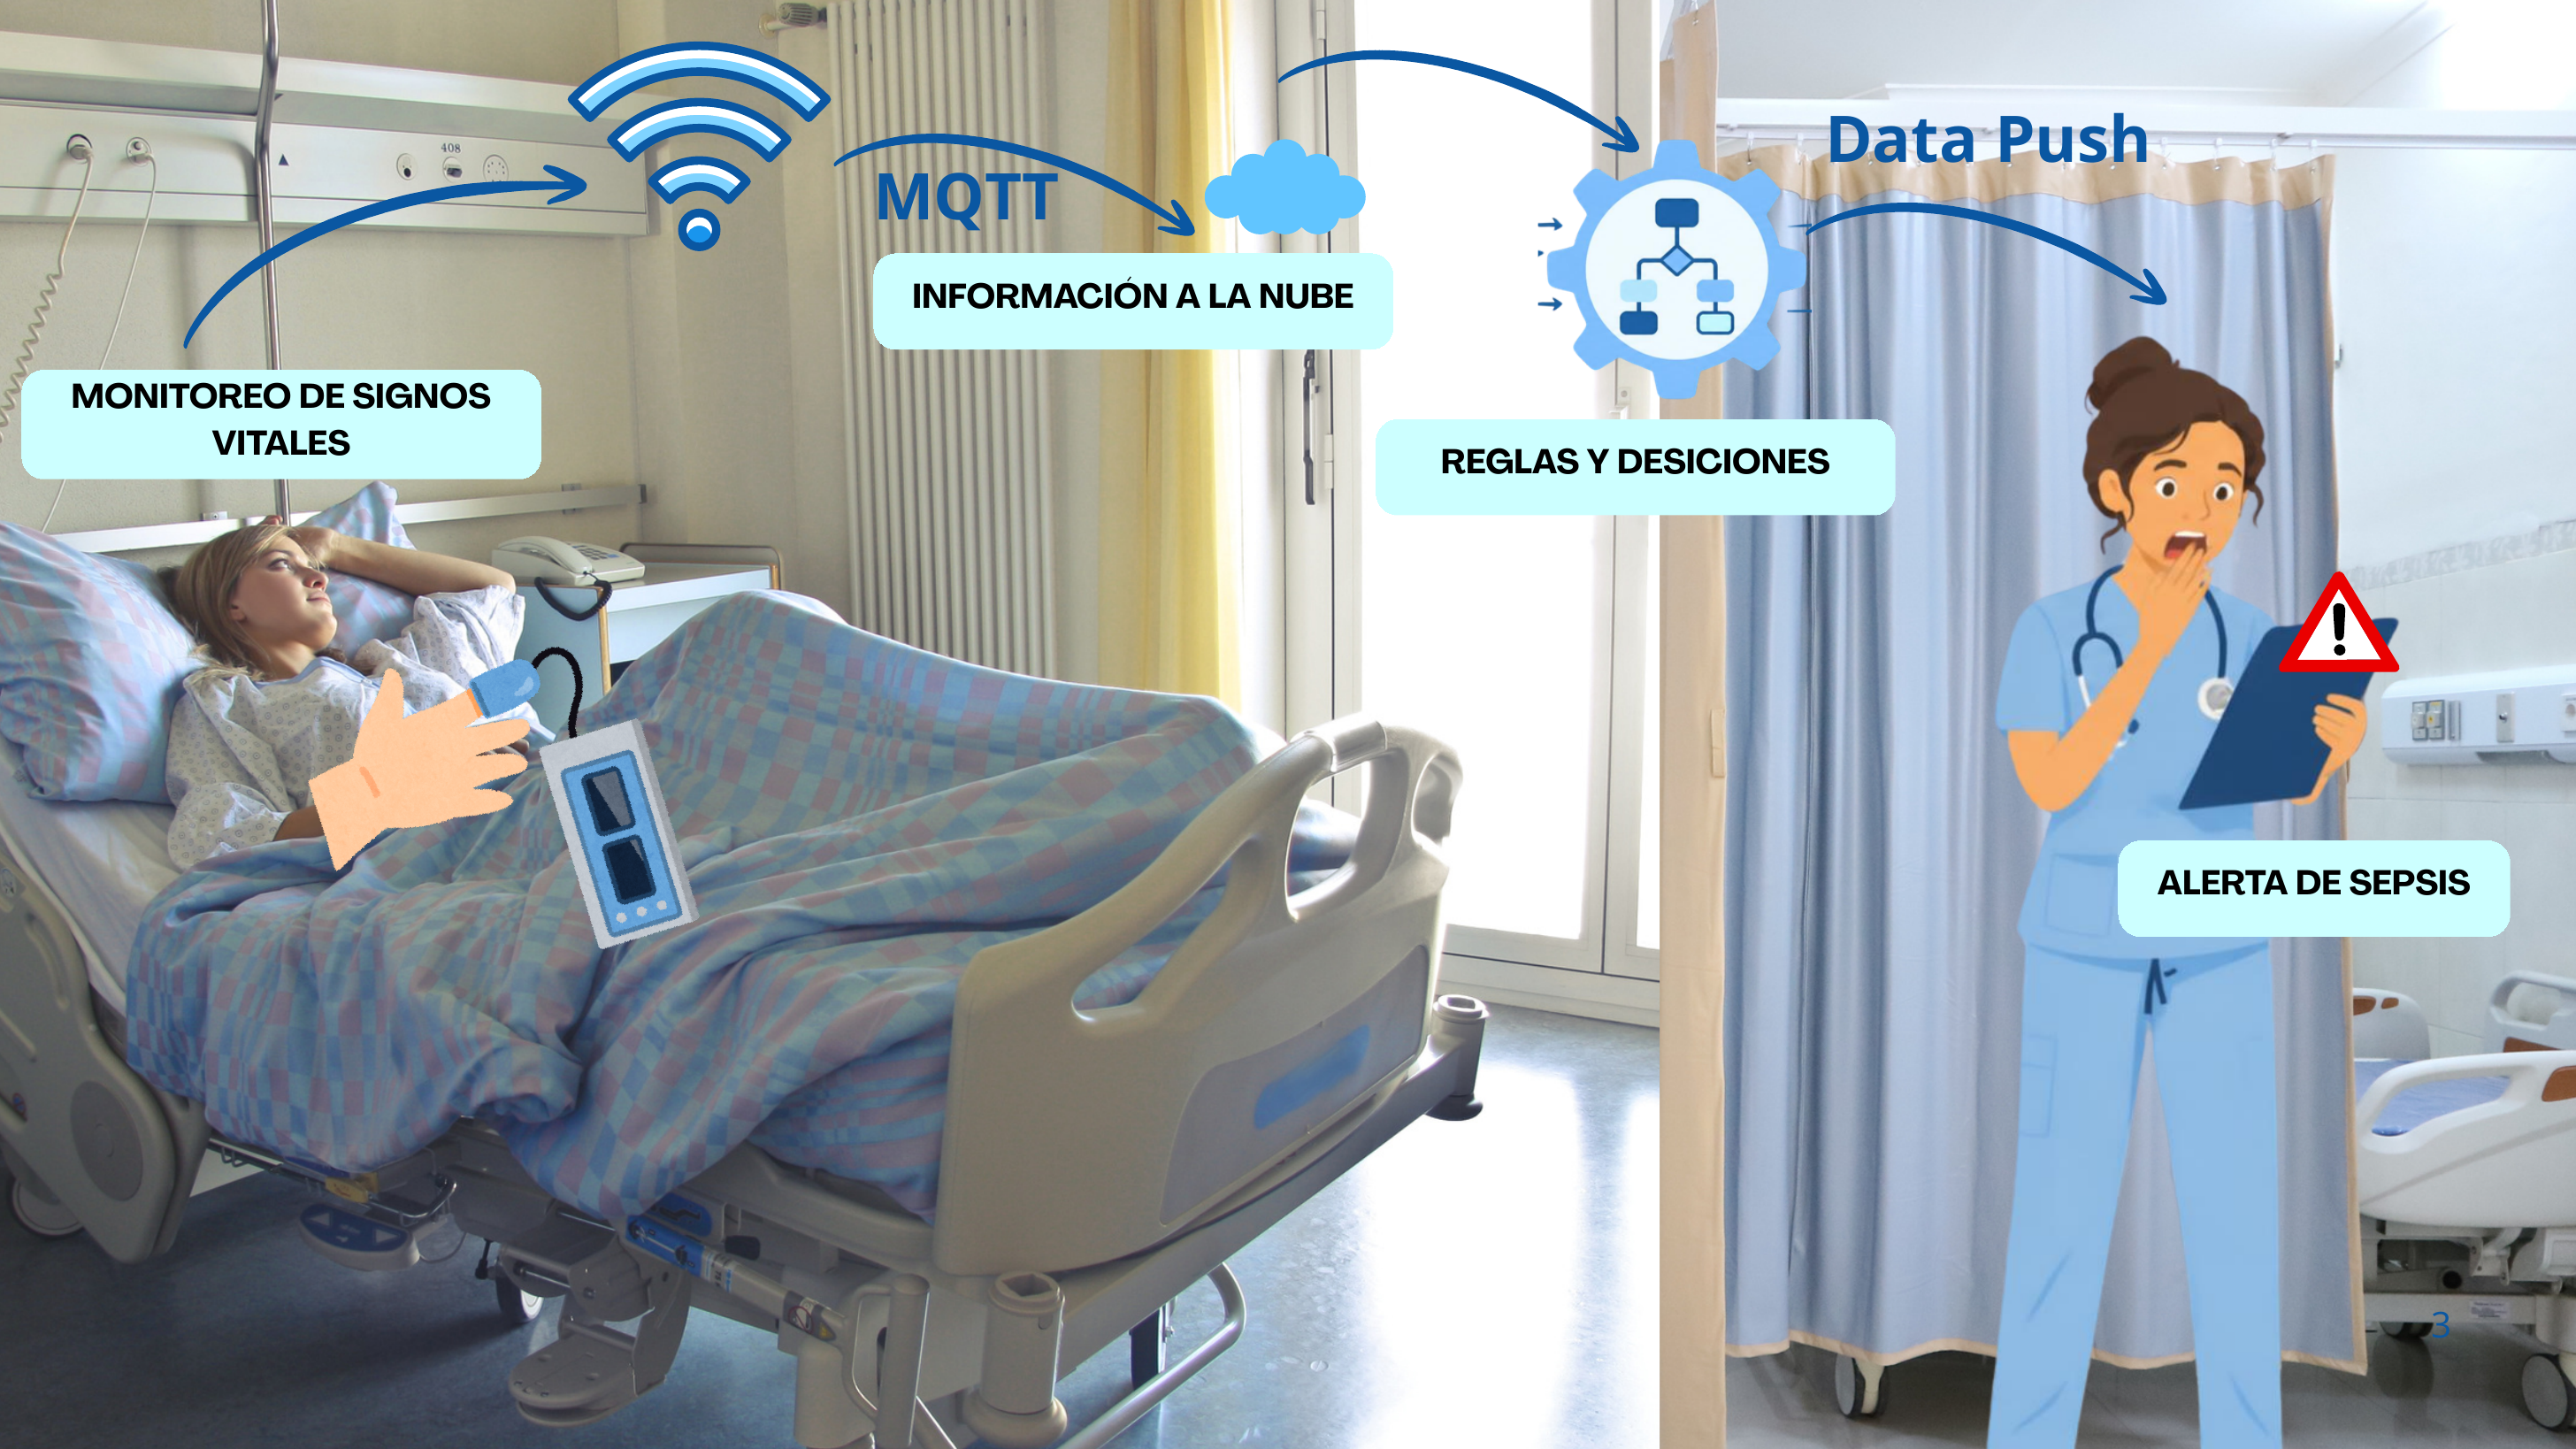
\includegraphics[width=0.85\linewidth]{vision_general.png}
    \caption{Funcionamiento general de la solución VIGIA.}
    \label{fig:vision_general}
\end{figure}

La solución implementada se organiza en una arquitectura IoT de cinco capas, en la que cada capa cumple una función específica y se comunica únicamente con las capas adyacentes. La Figura \ref{fig:arquitectura} presenta el diagrama de concepto, que agrupa estas capas en tres bloques: el nodo IoT (capas de percepción y borde), el \textit{broker} MQTT de ThingSpeak (capas de red y nube) y la aplicación móvil (capa de aplicación). La Tabla \ref{tab:capas} resume los componentes y tecnologías de cada capa.

\begin{figure}[H]
    \centering
    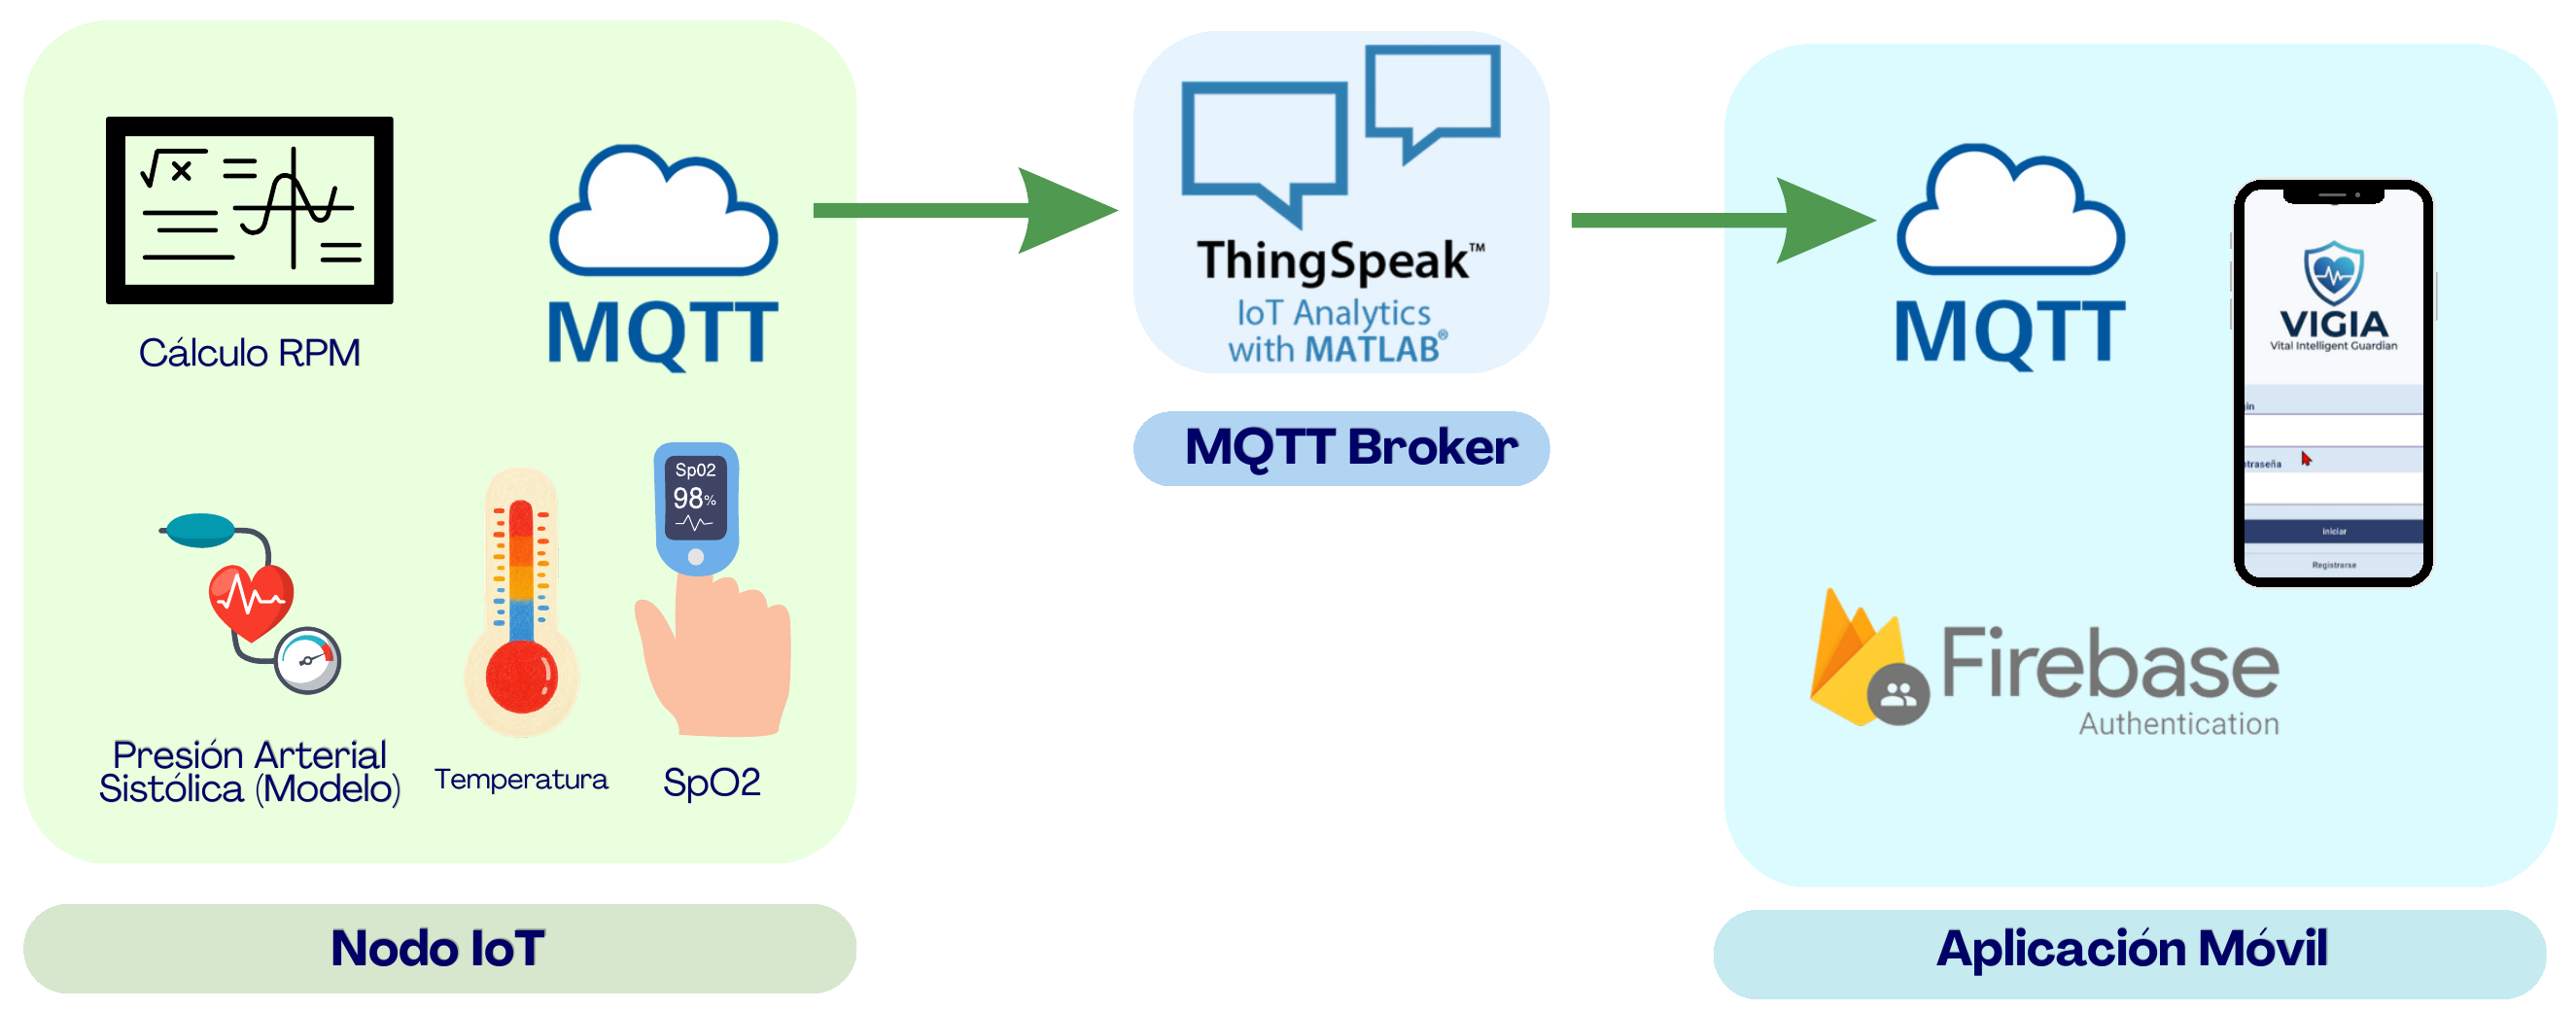
\includegraphics[width=0.9\linewidth]{arquitectura.png}
    \caption{Diagrama de concepto de la solución VIGIA.}
    \label{fig:arquitectura}
\end{figure}

\begin{enumerate}
    \item \textbf{Capa de percepción.} Está conformada por los sensores que interactúan directamente con el paciente: el MAX30100, que obtiene la señal PPG infrarroja y roja al colocar el dedo sobre el sensor, y el MLX90614, que mide la temperatura corporal sin contacto. Ambos sensores digitalizan la información y la entregan a la Raspberry Pi mediante el protocolo I2C.

    \item \textbf{Capa de borde (procesamiento local).} La Raspberry Pi 3 lee los sensores y procesa las señales en el mismo nodo, sin depender de la nube. A partir de la señal PPG obtiene la frecuencia cardíaca, la saturación de oxígeno, la frecuencia respiratoria y, mediante el clasificador \textit{Random Forest}, los puntos NEWS-2 de presión arterial sistólica. Con estos parámetros y la temperatura calcula el puntaje NEWS-2 total y su nivel de riesgo, y empaqueta cada lectura en formato SenML, que además se guarda localmente como respaldo.

    \item \textbf{Capa de red (transmisión).} La Raspberry Pi se conecta a internet por WiFi y publica las lecturas mediante el protocolo MQTT, bajo el patrón publicador/suscriptor, hacia el \textit{broker} de ThingSpeak. La conexión se realiza por el puerto 8883 con cifrado TLS y se autentica con credenciales de dispositivo MQTT. Cada variable se publica en su propio tópico (\textit{channels/<ID>/publish/fields/fieldN}), enviando un campo por mensaje en rotación y respetando un intervalo mínimo de 15 segundos entre mensajes, que es el límite de escritura de la plataforma.

    \item \textbf{Capa de nube (almacenamiento).} ThingSpeak almacena las lecturas en un canal de ocho campos: frecuencia cardíaca, SpO\textsubscript{2}, temperatura, frecuencia respiratoria, puntos de presión arterial, puntaje NEWS-2 total, identificador del nodo y marca de tiempo de la lectura en la Raspberry Pi. Cada dato queda guardado con su hora de recepción, lo cual permite consultar el histórico y observar tendencias, y está disponible mediante una API REST.

    \item \textbf{Capa de aplicación.} La aplicación móvil Android, desarrollada en Kotlin con Jetpack Compose, consulta la API REST de ThingSpeak cada 10 segundos, presenta los signos vitales y el puntaje NEWS-2 al personal médico, muestra el histórico y genera la alerta crítica cuando corresponde. El inicio de sesión y el registro de usuarios se realizan con Firebase Authentication, que se usa únicamente para la gestión de cuentas; los datos del paciente no se almacenan en Firebase.
\end{enumerate}

\begin{table}[H]
\centering
\small
\begin{tabular}{>{\raggedright}p{2.6cm} >{\raggedright}p{5.2cm} p{6cm}}
\toprule
\textbf{Capa} & \textbf{Componentes} & \textbf{Tecnologías / protocolos} \\
\midrule
Percepción & MAX30100, MLX90614 & I2C \\
Borde & Raspberry Pi 3 & Python, scikit-learn (\textit{Random Forest}), SenML \\
Red & WiFi, \textit{broker} MQTT & MQTT sobre TLS (puerto 8883) \\
Nube & Canal ThingSpeak (8 campos) & API REST (JSON) \\
Aplicación & App móvil VIGIA & Kotlin, Jetpack Compose, Firebase Authentication \\
\bottomrule
\end{tabular}
\caption{Componentes y tecnologías por capa.}
\label{tab:capas}
\end{table}



\subsection{Descripción de la capa de adquisición de datos}

La capa de adquisición está conformada por el nodo IoT, encargado de leer los sensores, procesar las señales de forma local y obtener los parámetros que requiere la escala NEWS-2. El nodo se construyó sobre una Raspberry Pi 3, que actúa como unidad de procesamiento y como pasarela hacia la nube, y dos sensores conectados al mismo bus I2C (bus 1 de la Raspberry Pi), cada uno con una dirección propia.

\subsubsection{Sensores}

La Tabla \ref{tab:sensores} resume los sensores del nodo, su dirección en el bus I2C, las variables que se obtienen de cada uno y la configuración utilizada.

\begin{table}[H]
\centering
\small
\begin{tabular}{>{\raggedright}p{2.2cm} >{\raggedright}p{1.6cm} >{\raggedright}p{3.6cm} p{6.2cm}}
\toprule
\textbf{Sensor} & \textbf{Dirección I2C} & \textbf{Variables} & \textbf{Configuración utilizada} \\
\midrule
MAX30100 & 0x57 & Señal PPG infrarroja y roja (BPM, SpO\textsubscript{2}, frecuencia respiratoria y presión arterial) & Modo SpO\textsubscript{2} (LED rojo e infrarrojo activos), 100 muestras/s, ancho de pulso de 1600~$\mu$s (ADC de 16 bits), misma corriente para ambos LED. \\
MLX90614 & 0x5A & Temperatura corporal sin contacto & Lectura del registro de temperatura del objeto, resolución de 0.02~°C y offset de calibración fijo de +1.48~°C. \\
\bottomrule
\end{tabular}
\caption{Sensores del nodo IoT.}
\label{tab:sensores}
\end{table}

El \textbf{MAX30100} es un sensor integrado de oximetría de pulso que emite luz roja e infrarroja sobre el dedo y mide, con un fotodetector, la cantidad de luz que se refleja. Cada vez que el corazón late, el volumen de sangre en los capilares cambia y con él la luz absorbida, lo cual produce la señal de fotopletismografía (PPG). Esta señal tiene dos componentes: una componente continua (DC), dominada por el tejido, el hueso y la sangre venosa, que cambia lentamente, y una componente alterna (AC), causada por el pulso arterial, que es la señal útil. Las muestras se almacenan en una memoria FIFO interna de solo 16 posiciones, equivalente a aproximadamente 160~ms de señal a 100 muestras/s, por lo que deben leerse de forma continua para no perder datos.

El \textbf{MLX90614} es un termómetro infrarrojo que mide la temperatura de la superficie hacia la que apunta sin necesidad de contacto. El valor del registro se convierte a grados Celsius como $T = 0.02 \cdot \text{raw} - 273.15$, y a este resultado se le suma el offset de calibración.

\subsubsection{Código implementado en la Raspberry Pi}

El código fue desarrollado en Python y se organiza en dos hilos de ejecución que comparten un estado protegido con un \textit{lock}. Esta separación responde a una restricción del MAX30100: como la FIFO solo almacena 160~ms de señal, ningún proceso pesado puede ejecutarse en el mismo ciclo en el que se lee el sensor. La Figura \ref{fig:flujo_rpi} presenta el diagrama de flujo del código.

\paragraph{Hilo principal: lectura de sensores.} Al iniciar se configuran ambos sensores, se carga el modelo de presión arterial y se configura la conexión MQTT. Luego, cada 5~ms se consulta cuántas muestras nuevas tiene la FIFO, comparando los punteros de escritura y lectura del MAX30100, y se leen todas las disponibles. Cada muestra (IR y roja) pasa por el procesador de señal y la muestra IR se guarda además en un \textit{buffer} circular de 60 segundos (6,000 muestras) que utiliza el hilo NEWS-2. Una vez por segundo se lee la temperatura, se calculan BPM y SpO\textsubscript{2} y se actualiza el estado compartido.

Para garantizar que la lectura no se detenga se implementaron tres mecanismos de recuperación de la FIFO: se vacía justo antes de empezar a leerla, ya que la carga del modelo puede tardar lo suficiente para desbordarla; se vacía de inmediato ante cualquier error de comunicación I2C; y un \textit{watchdog} la vacía si pasa más de 1 segundo sin recibir muestras nuevas, situación en la que el sensor queda bloqueado con ambos punteros iguales.

\paragraph{Separación de componentes y detección de latidos.} La componente DC de cada canal se estima con una media móvil exponencial (EMA) de coeficiente $\alpha = 0.03$, que sigue los cambios lentos de la señal, y la componente AC se obtiene restándola de la muestra:
\begin{equation}
    DC_k = DC_{k-1} + \alpha\,(x_k - DC_{k-1}), \qquad AC_k = x_k - DC_k
\end{equation}

Sobre la componente AC infrarroja se detectan los latidos con un umbral adaptativo igual al 55\% de la amplitud reciente del pulso (calculada sobre las últimas 20 muestras y suavizada), de forma que el detector se ajusta a la intensidad de la señal de cada persona. Para evitar contar dos veces el mismo latido se usa histéresis: tras detectar un latido, el detector solo se rearma cuando la señal baja del 40\% del umbral durante 5 muestras consecutivas, y además se exige un periodo refractario de 0.33~s.

\paragraph{Frecuencia cardíaca.} Solo se aceptan intervalos entre latidos de 0.33 a 1.8~s (33 a 180~lpm), y se descarta cualquier intervalo que se desvíe más de un 40\% de la mediana de los anteriores, lo cual elimina latidos mal detectados por movimiento. El BPM se calcula como $60/\tilde{T}$, donde $\tilde{T}$ es la mediana de los últimos 8 intervalos válidos, y se suaviza con una EMA (70\% valor previo, 30\% valor nuevo). Si pasan más de 3 segundos sin detectar un latido se asume que el dedo fue retirado y la medición se reinicia.

\paragraph{Saturación de oxígeno.} Se calcula la razón de razones entre los canales rojo e infrarrojo, utilizando el valor RMS de las últimas 200 muestras AC de cada canal y normalizando por su componente DC, para que el resultado no dependa del grosor del dedo ni de la intensidad de los LED:
\begin{equation}
    R = \frac{AC_{rms,rojo}/DC_{rojo}}{AC_{rms,IR}/DC_{IR}}, \qquad SpO_2 = 110 - 25R
\end{equation}
El resultado se limita al rango de 70 a 100\% y se suaviza con una EMA (85\% valor previo, 15\% valor nuevo). Si la señal infrarroja es demasiado débil ($AC_{rms,IR} < 15$) no se actualiza el valor.

\paragraph{Hilo NEWS-2: frecuencia respiratoria, presión arterial y puntaje.} Cada 10 segundos este hilo copia el estado compartido y el \textit{buffer} de 60 segundos de señal IR. La frecuencia respiratoria se obtiene aislando la modulación respiratoria de la señal PPG con un filtro pasa-banda Butterworth de 0.1 a 0.5~Hz (6 a 30 respiraciones por minuto) y contando los picos de la señal filtrada en la ventana; el valor solo se acepta si se encuentra dentro de ese rango y se dispone de al menos 20 segundos de señal. Los puntos de presión arterial se obtienen con el clasificador descrito en la capa de analítica, y con todos los parámetros se calcula el puntaje NEWS-2. Finalmente, la lectura se empaqueta en formato SenML, se guarda en un archivo local y se entrega al módulo de transmisión.

Las lecturas que no son válidas (por ejemplo, BPM o SpO\textsubscript{2} iguales a cero cuando no hay dedo, o temperatura no disponible si el MLX90614 no responde) se reportan como vacías en lugar de enviarse como valores reales. Adicionalmente, el nodo guarda localmente un registro de cada lectura por segundo, lo cual permite revisar la sesión aunque falle la conexión.

\begin{figure}[H]
\centering
\resizebox{\textwidth}{!}{%
\begin{tikzpicture}[
    node distance=0.35cm and 0.6cm,
    proc/.style={draw, rounded corners, fill=blue!6, align=center, text width=5.6cm, font=\scriptsize, minimum height=0.7cm},
    dec/.style={draw, diamond, aspect=2.6, fill=yellow!15, align=center, font=\scriptsize, inner sep=0pt, text width=2.2cm},
    term/.style={draw, rounded corners=8pt, fill=green!12, align=center, font=\scriptsize\bfseries, text width=3cm, minimum height=0.6cm},
    hilo/.style={draw, rounded corners, fill=orange!10, align=center, text width=4.6cm, font=\scriptsize, minimum height=0.7cm},
    arr/.style={-{Stealth}, thick},
    lab/.style={font=\scriptsize}
]
% ---------------- Hilo principal ----------------
\node[term] (ini) {Hilo principal};
\node[proc, below=of ini] (i2c) {Abrir bus I2C 1: MLX90614 (0x5A) y MAX30100 (0x57) \\ reset, modo SpO\textsubscript{2}, 100 muestras/s, corriente LED};
\node[proc, below=of i2c] (carga) {Cargar clasificador PA, configurar MQTT, \\ abrir archivo SenML local};
\node[proc, below=of carga] (lanza) {Lanzar hilo NEWS-2 y vaciar FIFO del MAX30100};
\node[proc, below=of lanza] (n) {Muestras pendientes: \\ \textit{n = (wr\_ptr - rd\_ptr) mod 16}};
\node[dec, below=of n] (d1) {¿n > 0?};
\node[proc, below=of d1] (lee) {Leer n muestras (IR, rojo) de la FIFO \\ Separar DC/AC (EMA), detectar latido \\ Guardar IR en \textit{buffer} de 60 s};
\node[dec, below=of lee] (d2) {¿Error I2C o > 1 s sin muestras?};
\node[proc, text width=2.3cm, left=0.6cm of d2] (flush) {Vaciar FIFO \\ (watchdog)};
\node[dec, below=of d2] (d3) {¿Pasó 1 s desde el último reporte?};
\node[proc, below=of d3] (rep) {Leer temperatura (MLX90614) \\ Calcular BPM y SpO\textsubscript{2} \\ Actualizar estado compartido (lock) \\ Mostrar y registrar lectura};
\node[proc, below=of rep] (esp) {Esperar 5 ms};

\draw[arr] (ini) -- (i2c);
\draw[arr] (i2c) -- (carga);
\draw[arr] (carga) -- (lanza);
\draw[arr] (lanza) -- (n);
\draw[arr] (n) -- (d1);
\draw[arr] (d1) -- node[lab, right]{Sí} (lee);
\draw[arr] (lee) -- (d2);
\draw[arr] (d1.east) -- node[lab, above]{No} ++(3.2,0) |- (d2.east);
\draw[arr] (d2.west) -- node[lab, above]{Sí} (flush.east);
\draw[arr] (flush.south) |- (d3.west);
\draw[arr] (d2) -- node[lab, right]{No} (d3);
\draw[arr] (d3) -- node[lab, right]{Sí} (rep);
\draw[arr] (d3.east) -- node[lab, above]{No} ++(3.2,0) |- (esp.east);
\draw[arr] (rep) -- (esp);
\draw[arr] (esp.west) -- ++(-2.4,0) |- (n.west);

% ---------------- Hilo NEWS-2 ----------------
\node[term] (h0) at (9.2,0) {Hilo NEWS-2};
\node[hilo, below=of h0] (h1) {Esperar 10 s};
\node[hilo, below=of h1] (h2) {Copiar estado compartido (BPM, SpO\textsubscript{2}, temperatura) y \textit{buffer} IR de 60 s};
\node[hilo, below=of h2] (h3) {Frecuencia respiratoria: pasa-banda 0.1--0.5 Hz y conteo de picos (6--30 rpm)};
\node[hilo, below=of h3] (h4) {Puntos NEWS-2 de presión arterial con el clasificador Random Forest};
\node[hilo, below=of h4] (h5) {Puntos por parámetro, puntaje NEWS-2 total y nivel de riesgo};
\node[hilo, below=of h5] (h6) {Empaquetar en SenML $\rightarrow$ guardar en archivo local $\rightarrow$ publicar a ThingSpeak (MQTT)};

\draw[arr] (h0) -- (h1);
\draw[arr] (h1) -- (h2);
\draw[arr] (h2) -- (h3);
\draw[arr] (h3) -- (h4);
\draw[arr] (h4) -- (h5);
\draw[arr] (h5) -- (h6);
\draw[arr] (h6.east) -- ++(0.4,0) |- (h1.east);

\draw[arr, dashed] (lanza.east) -- node[lab, above, pos=0.3]{crea} ++(3.6,0) |- (h0.west);
\end{tikzpicture}%
}
\caption{Diagrama de flujo del código implementado en la Raspberry Pi 3.}
\label{fig:flujo_rpi}
\end{figure}


\subsection{Descripción de la transmisión de datos}

La transmisión de datos se realiza en dos tramos: desde el nodo IoT hacia la nube, mediante el protocolo MQTT, y desde la nube hacia la aplicación, mediante la API REST de ThingSpeak. La Raspberry Pi se conecta a internet a través de la red WiFi del lugar de despliegue.

\subsubsection{Formato de los datos: SenML}

Cada lectura que genera el hilo NEWS-2 se representa en formato SenML (\textit{Sensor Measurement Lists}, RFC 8428), un estándar para describir mediciones de sensores en JSON. El primer registro de cada lectura contiene los campos base, que son compartidos por todos los demás: el nombre base del nodo (\textit{bn}), la marca de tiempo base en época Unix (\textit{bt}) y la versión de SenML (\textit{bver}). Cada registro contiene además el nombre de la variable (\textit{n}), su unidad (\textit{u}) cuando aplica y su valor (\textit{v}). Las variables sin lectura válida no se incluyen en el mensaje. La Tabla \ref{tab:senml} presenta un ejemplo de una lectura en este formato.

\begin{table}[H]
\centering
\small
\begin{tabular}{l l l}
\toprule
\textbf{Nombre (\textit{n})} & \textbf{Unidad (\textit{u})} & \textbf{Valor (\textit{v})} \\
\midrule
\textit{max30100:hr} & 1/min & 78 \\
\textit{max30100:spo2} & \% & 97 \\
\textit{mlx90614:temp} & Cel & 36.6 \\
\textit{resp\_rate} & 1/min & 16 \\
\textit{sbp\_news2\_points} & -- & 0 \\
\textit{news2\_total} & -- & 0 \\
\textit{news2\_level} & -- & 0 \\
\textit{node\_id} & -- & pi3-001 \\
\textit{timestamp} & s & 1794236400 \\
\bottomrule
\end{tabular}
\caption{Ejemplo de una lectura en formato SenML. El primer registro incluye además los campos base: \textit{bn} = \textit{urn:dev:pi3-001:}, \textit{bt} (marca de tiempo de la lectura) y \textit{bver} = 5, junto con el campo auxiliar \textit{bt\_legible}, que no forma parte del estándar y solo facilita la lectura humana del archivo local.}
\label{tab:senml}
\end{table}

Cada lectura en SenML se guarda también en un archivo local (una línea JSON por lectura), lo cual sirve como respaldo cuando no hay conexión.

\subsubsection{Nodo IoT hacia la nube: MQTT}

El nodo publica los datos con el protocolo MQTT, bajo el patrón publicador/suscriptor, hacia el \textit{broker} de ThingSpeak (\textit{mqtt3.thingspeak.com}). La comunicación se protege con TLS en el puerto 8883, verificando el certificado del servidor, y el nodo se autentica con las credenciales de un dispositivo MQTT registrado en ThingSpeak (identificador de cliente, usuario y contraseña), que son distintas de las llaves de la API del canal y se almacenan en un archivo de configuración que no se incluye en el repositorio. Los mensajes se envían con calidad de servicio QoS 0.

Se utiliza un tópico por variable, con el formato que define ThingSpeak, y el contenido de cada mensaje es el valor de la variable tomado del registro SenML correspondiente. La Tabla \ref{tab:topicos} presenta la asignación de variables a campos del canal.

\begin{table}[H]
\centering
\footnotesize
\begin{tabular}{l l l}
\toprule
\textbf{Tópico MQTT} & \textbf{Variable (SenML)} & \textbf{Descripción} \\
\midrule
\textit{channels/<ID>/publish/fields/field1} & \textit{max30100:hr} & Frecuencia cardíaca (lpm) \\
\textit{channels/<ID>/publish/fields/field2} & \textit{max30100:spo2} & SpO\textsubscript{2} (\%) \\
\textit{channels/<ID>/publish/fields/field3} & \textit{mlx90614:temp} & Temperatura corporal (°C) \\
\textit{channels/<ID>/publish/fields/field4} & \textit{resp\_rate} & Frecuencia respiratoria (rpm) \\
\textit{channels/<ID>/publish/fields/field5} & \textit{sbp\_news2\_points} & Puntos NEWS-2 de presión arterial \\
\textit{channels/<ID>/publish/fields/field6} & \textit{news2\_total} & Puntaje NEWS-2 total \\
\textit{channels/<ID>/publish/fields/field7} & \textit{node\_id} & Identificador del nodo \\
\textit{channels/<ID>/publish/fields/field8} & \textit{timestamp} & Hora de la lectura en la Raspberry Pi \\
\bottomrule
\end{tabular}
\caption{Asignación de variables a los campos del canal de ThingSpeak.}
\label{tab:topicos}
\end{table}

La Figura \ref{fig:thingspeak} muestra la configuración de los ocho campos en el canal de ThingSpeak, junto con la salida de la consola de la Raspberry Pi al enviar un mensaje y el indicador de conexión del nodo en la aplicación, que pasa a \textit{No conectado} cuando deja de recibir datos.

\begin{figure}[H]
    \centering
    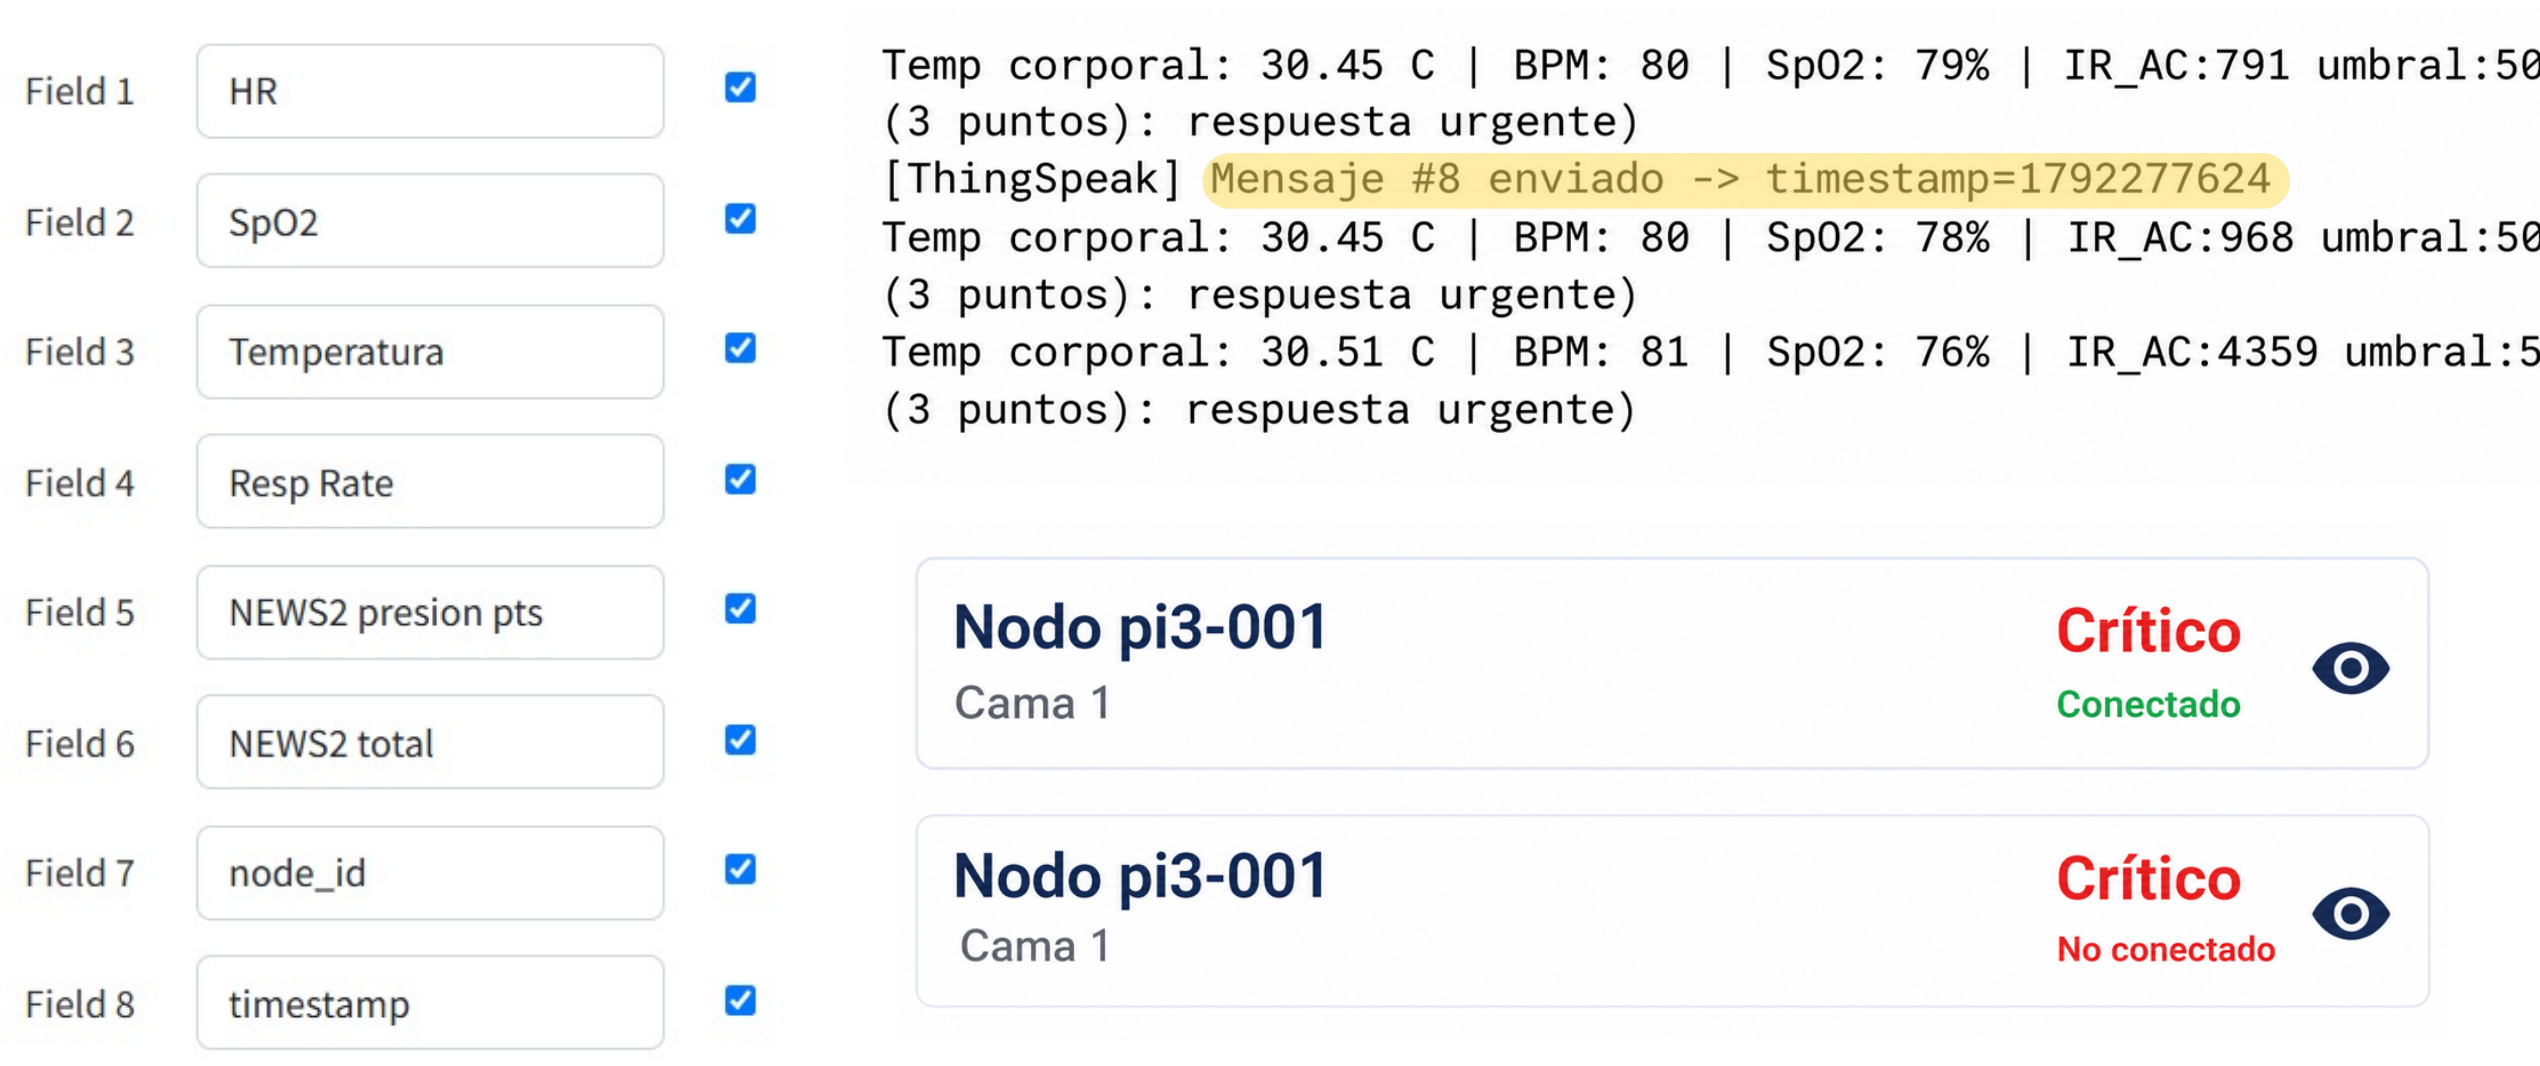
\includegraphics[width=0.95\linewidth]{thingspeak_campos.png}
    \caption{Campos del canal de ThingSpeak, envío de mensajes desde la Raspberry Pi y estado de conexión del nodo en la aplicación.}
    \label{fig:thingspeak}
\end{figure}

ThingSpeak admite como máximo una escritura por canal cada 15 segundos en su versión gratuita. Por esta razón cada mensaje lleva un solo campo y los campos se envían en rotación: en cada envío se publica el siguiente campo de la lista que tenga un valor válido. El hilo NEWS-2 intenta publicar cada 10 segundos, pero el envío solo se realiza si han pasado al menos 15 segundos desde el anterior, por lo que en la práctica se publica un campo cada 20 segundos. Para que la aplicación pueda saber cuándo se tomó realmente la lectura, y no solo cuándo llegó a la nube, el nodo envía también su propia marca de tiempo en el campo 8.

\subsubsection{Nube hacia la aplicación: API REST}

ThingSpeak almacena cada mensaje con su hora de recepción. La aplicación consulta los datos mediante peticiones HTTPS GET a la API REST del canal, autenticadas con la llave de lectura, y recibe la respuesta en formato JSON. Cada 10 segundos solicita las últimas 30 entradas del canal para obtener el estado actual del paciente; como cada entrada contiene un solo campo, la aplicación recorre las entradas de la más reciente a la más antigua y toma el primer valor no vacío de cada campo. Para la gráfica del histórico NEWS-2 y el registro de alertas se solicitan las últimas 200 entradas.

\subsection{Descripción de la capa de aplicación y analítica de datos}

La analítica de datos de la solución se encuentra distribuida en dos niveles. En el borde, la Raspberry Pi 3 ejecuta el modelo de aprendizaje automático que clasifica el nivel de riesgo de la presión arterial sistólica a partir de la señal PPG y calcula el puntaje NEWS-2 agregado con los demás signos vitales. En la capa de aplicación, la app móvil consulta los datos almacenados en ThingSpeak, traduce cada parámetro a su categoría de riesgo y genera la alerta crítica cuando el paciente cumple los criterios de escalamiento de la escala. A continuación se describe en detalle el componente central de la analítica: el clasificador de riesgo de presión arterial.

\subsubsection{Conjunto de datos de entrenamiento}

El modelo fue entrenado con el \textit{dataset} público \textit{Cuff-Less Blood Pressure Estimation} de Kachuee/UCI \cite{ref22}, derivado de la base de datos MIMIC-II. El \textit{dataset} está compuesto por 12,000 registros de aproximadamente 8 minutos cada uno, muestreados a 125~Hz, y cada registro contiene tres canales sincronizados: la señal PPG, la presión arterial invasiva (ABP) en mmHg, que se utiliza como valor de referencia real, y la señal ECG, la cual no se utiliza en este trabajo ya que el nodo IoT únicamente cuenta con el sensor MAX30100.

Los 12,000 registros provienen de 942 pacientes, sin embargo el identificador de paciente fue suprimido al publicar el \textit{dataset} y no se incluyen datos demográficos (edad, sexo, peso o altura). Por esta razón, la separación entre datos de entrenamiento y de prueba se realizó a nivel de registro, que es el nivel de agrupamiento más fino disponible, garantizando que ningún registro aparezca simultáneamente en ambos conjuntos.

\subsubsection{Extracción de características morfológicas}

Sobre cada registro se aplica el mismo procesamiento que posteriormente se ejecuta en tiempo real sobre la señal del MAX30100, lo cual asegura que el modelo reciba en operación el mismo tipo de información con el que fue entrenado. La Figura \ref{fig:pipeline_ppg} resume las primeras etapas: la señal PPG se compone de una componente DC, que no interesa, y una componente AC, que corresponde a cada latido; el filtro pasa-banda elimina la línea base y el ruido, y luego se identifican en cada latido su inicio, su pico y el inicio del siguiente. El proceso completo se divide en las siguientes etapas:

\begin{figure}[H]
    \centering
    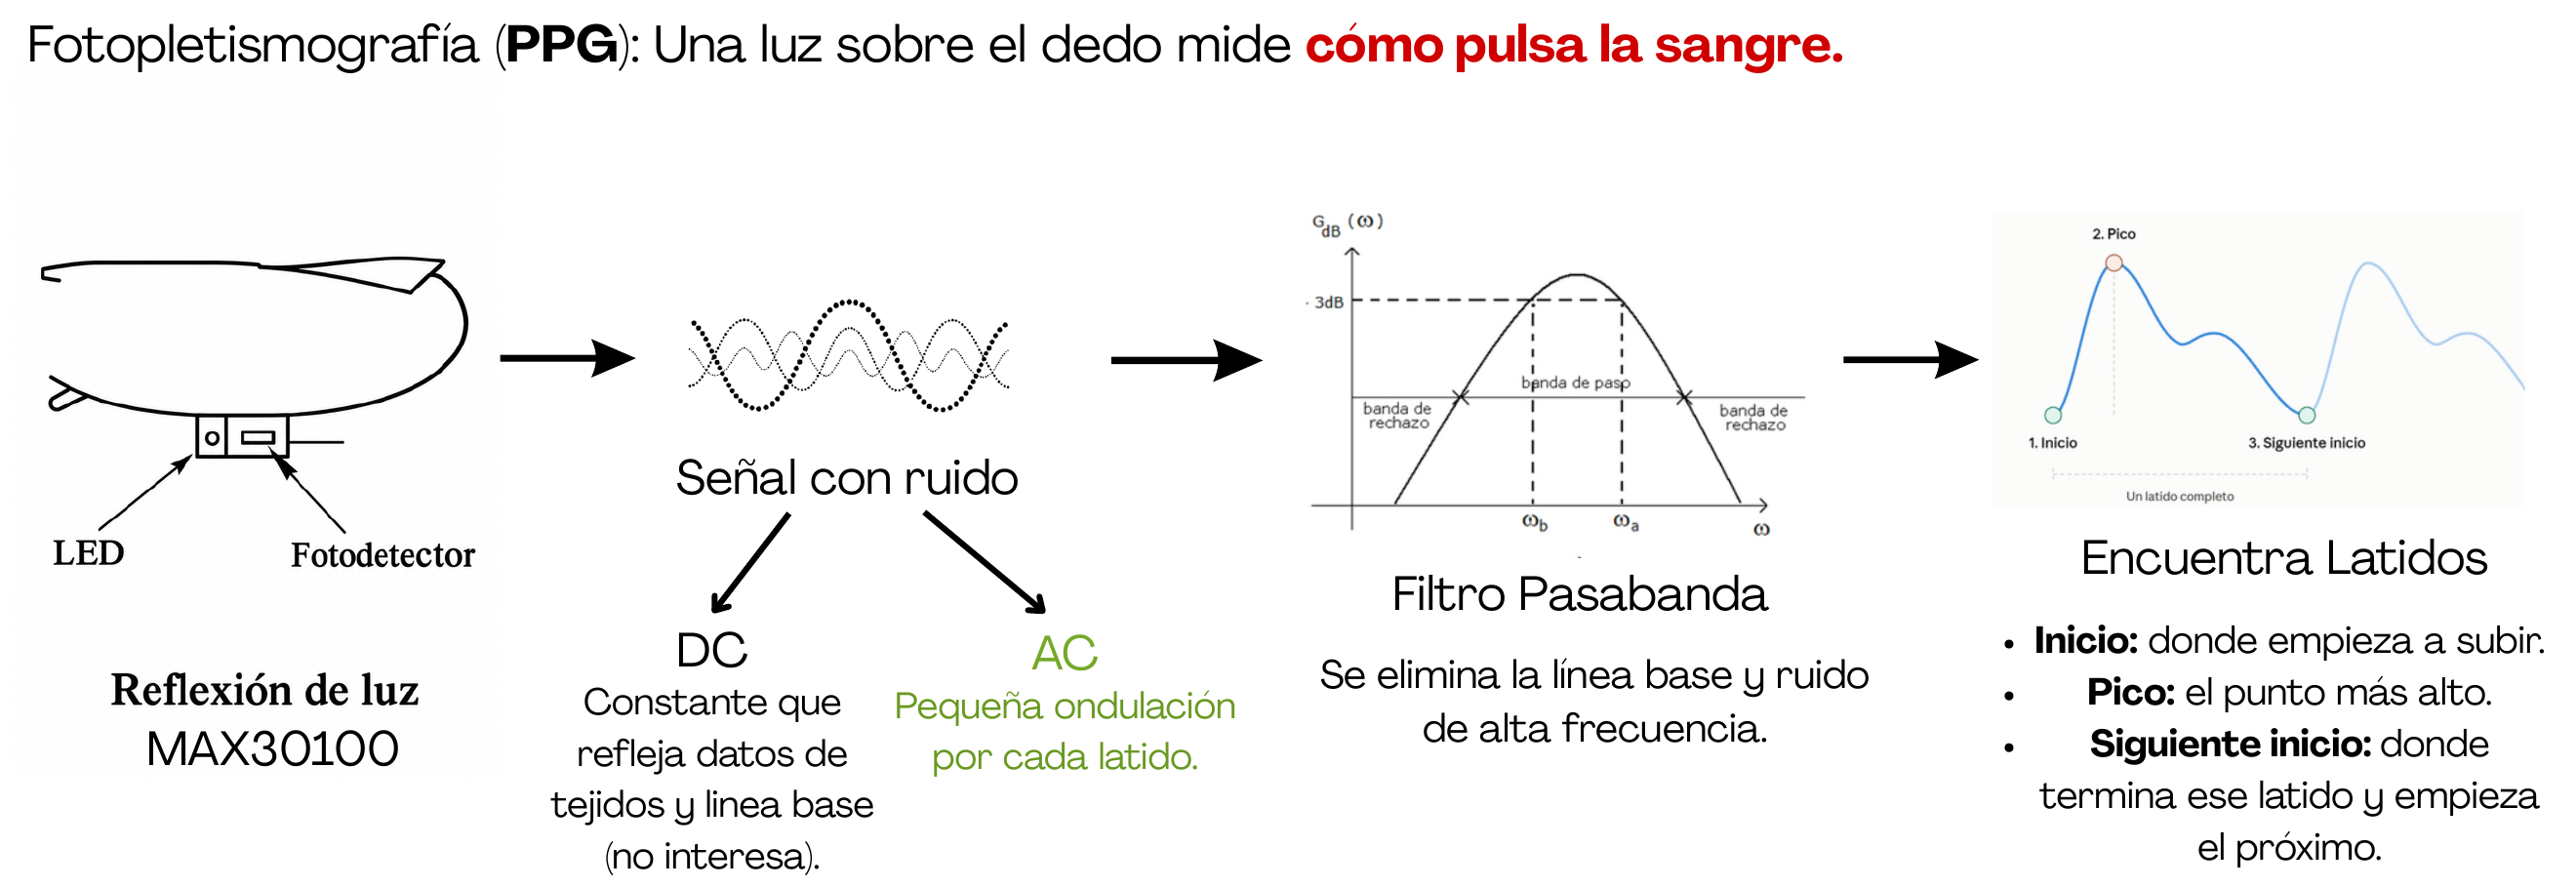
\includegraphics[width=0.95\linewidth]{pipeline_ppg.png}
    \caption{Adquisición de la señal PPG, filtrado y detección de latidos.}
    \label{fig:pipeline_ppg}
\end{figure}

\begin{enumerate}
    \item Se aplica un filtro pasa-banda Butterworth de orden 4 entre 0.5 y 8~Hz, con filtrado de fase cero, para eliminar la deriva de la línea base y el ruido de alta frecuencia sin deformar la morfología del pulso.
    \item Se detectan los ciclos de pulso identificando para cada latido el inicio de la onda (\textit{onset}), el pico sistólico y el inicio del siguiente ciclo. Solo se aceptan ciclos con una frecuencia cardíaca entre 40 y 180~lpm.
    \item Se aplican filtros de calidad: los anchos del pulso al 25, 50 y 75\% de su amplitud deben decrecer de forma monotónica (lo cual descarta pulsos deformados), y se eliminan los ciclos con amplitud o duración atípicas mediante un \textit{z-score} robusto basado en la mediana de las desviaciones absolutas (MAD) con umbral de 4. En el entrenamiento se descartan además los ciclos cuya presión de referencia no se encuentra en un rango fisiológico (sistólica 70--200~mmHg, diastólica 40--130~mmHg, presión de pulso 20--100~mmHg).
    \item De cada ciclo válido se extraen las 15 características morfológicas de la Tabla \ref{tab:features}.
    \item Las características se agrupan en ventanas de 10 ciclos consecutivos, tomando la mediana de cada una, lo cual reduce la variabilidad latido a latido y el efecto de ciclos ruidosos aislados. Se conservan hasta 15 ventanas por registro, distribuidas uniformemente a lo largo de este.
\end{enumerate}

\begin{table}[H]
\centering
\small
\begin{tabular}{>{\raggedright}p{3.3cm} p{10.5cm}}
\toprule
\textbf{Característica} & \textbf{Descripción} \\
\midrule
\textit{rise\_time} & Tiempo entre el inicio del pulso y el pico sistólico. \\
\textit{width\_25/50/75} & Ancho del pulso al 25, 50 y 75\% de su amplitud. \\
\textit{notch\_time} & Tiempo entre el pico sistólico y la muesca dicrótica. \\
\textit{amplitude} & Amplitud del pulso (pico menos inicio). \\
\textit{max\_d1} & Máximo de la primera derivada (velocidad de subida). \\
\textit{max\_d2}, \textit{min\_d2} & Máximo y mínimo de la segunda derivada (aceleración). \\
\textit{d2\_ratio} & Razón entre el mínimo y el máximo de la segunda derivada. \\
\textit{heart\_rate} & Frecuencia cardíaca instantánea del ciclo. \\
\textit{area\_ratio} & Razón entre el área sistólica y el área diastólica del pulso. \\
\textit{notch\_depth\_ratio} & Profundidad relativa de la muesca dicrótica. \\
\textit{aug\_index} & Índice de aumentación (altura de la onda reflejada respecto a la amplitud). \\
\textit{spectral\_ratio} & Razón entre el segundo y el primer armónico de la FFT del ciclo. \\
\bottomrule
\end{tabular}
\caption{Características morfológicas extraídas de cada ciclo de pulso PPG.}
\label{tab:features}
\end{table}

Como resultado se obtuvo un \textit{dataset} de 119,880 ventanas pertenecientes a 11,022 registros.

\subsubsection{De la estimación en mmHg a la clasificación del riesgo NEWS-2}

Inicialmente, tal como se planteó al comienzo del proyecto, se entrenó un \textit{Random Forest Regressor} para estimar directamente el valor de presión sistólica en mmHg. Sin embargo, como se detalla en la sección de resultados, la estimación absoluta a partir de PPG de un solo sensor, sin calibración por paciente, no cumple con el estándar AAMI \cite{ref23}, y al convertir sus predicciones a puntos NEWS-2 el modelo tiende a predecir valores cercanos a la media, dejando sin detectar la mayoría de los casos extremos, que son precisamente los de mayor interés clínico.

Dado que la escala NEWS-2 no utiliza el valor exacto de la presión sino el rango en el que se encuentra (Tabla \ref{tab:news2_pa}), se reformuló el problema como una clasificación del puntaje de riesgo de presión sistólica en lugar de una regresión continua.

\begin{table}[H]
\centering
\begin{tabular}{cc}
\toprule
\textbf{Presión sistólica (mmHg)} & \textbf{Puntos NEWS-2} \\
\midrule
$\leq 90$ & 3 \\
91--100 & 2 \\
101--110 & 1 \\
111--219 & 0 \\
$\geq 220$ & 3 \\
\bottomrule
\end{tabular}
\caption{Puntuación NEWS-2 de la presión arterial sistólica \cite{ref26}.}
\label{tab:news2_pa}
\end{table}

\subsubsection{Clasificador de riesgo de presión arterial}

El modelo implementado es un \textit{Random Forest Classifier} multiclase que predice directamente los puntos NEWS-2 de la presión sistólica (0, 1, 2 o 3). La Figura \ref{fig:modelo_rf} resume su funcionamiento: tras descartar los latidos anormales, de la forma de cada latido se calculan las 15 características, que se entregan a los 300 árboles de decisión, y el resultado final son los puntos de riesgo de presión sistólica. Durante el entrenamiento, cada conjunto de 15 características se asoció a la presión real medida con catéter, de modo que el modelo aprendió qué formas de pulso corresponden a cada nivel de riesgo; ya entrenado, solo necesita la señal que entrega el sensor.

\begin{figure}[H]
    \centering
    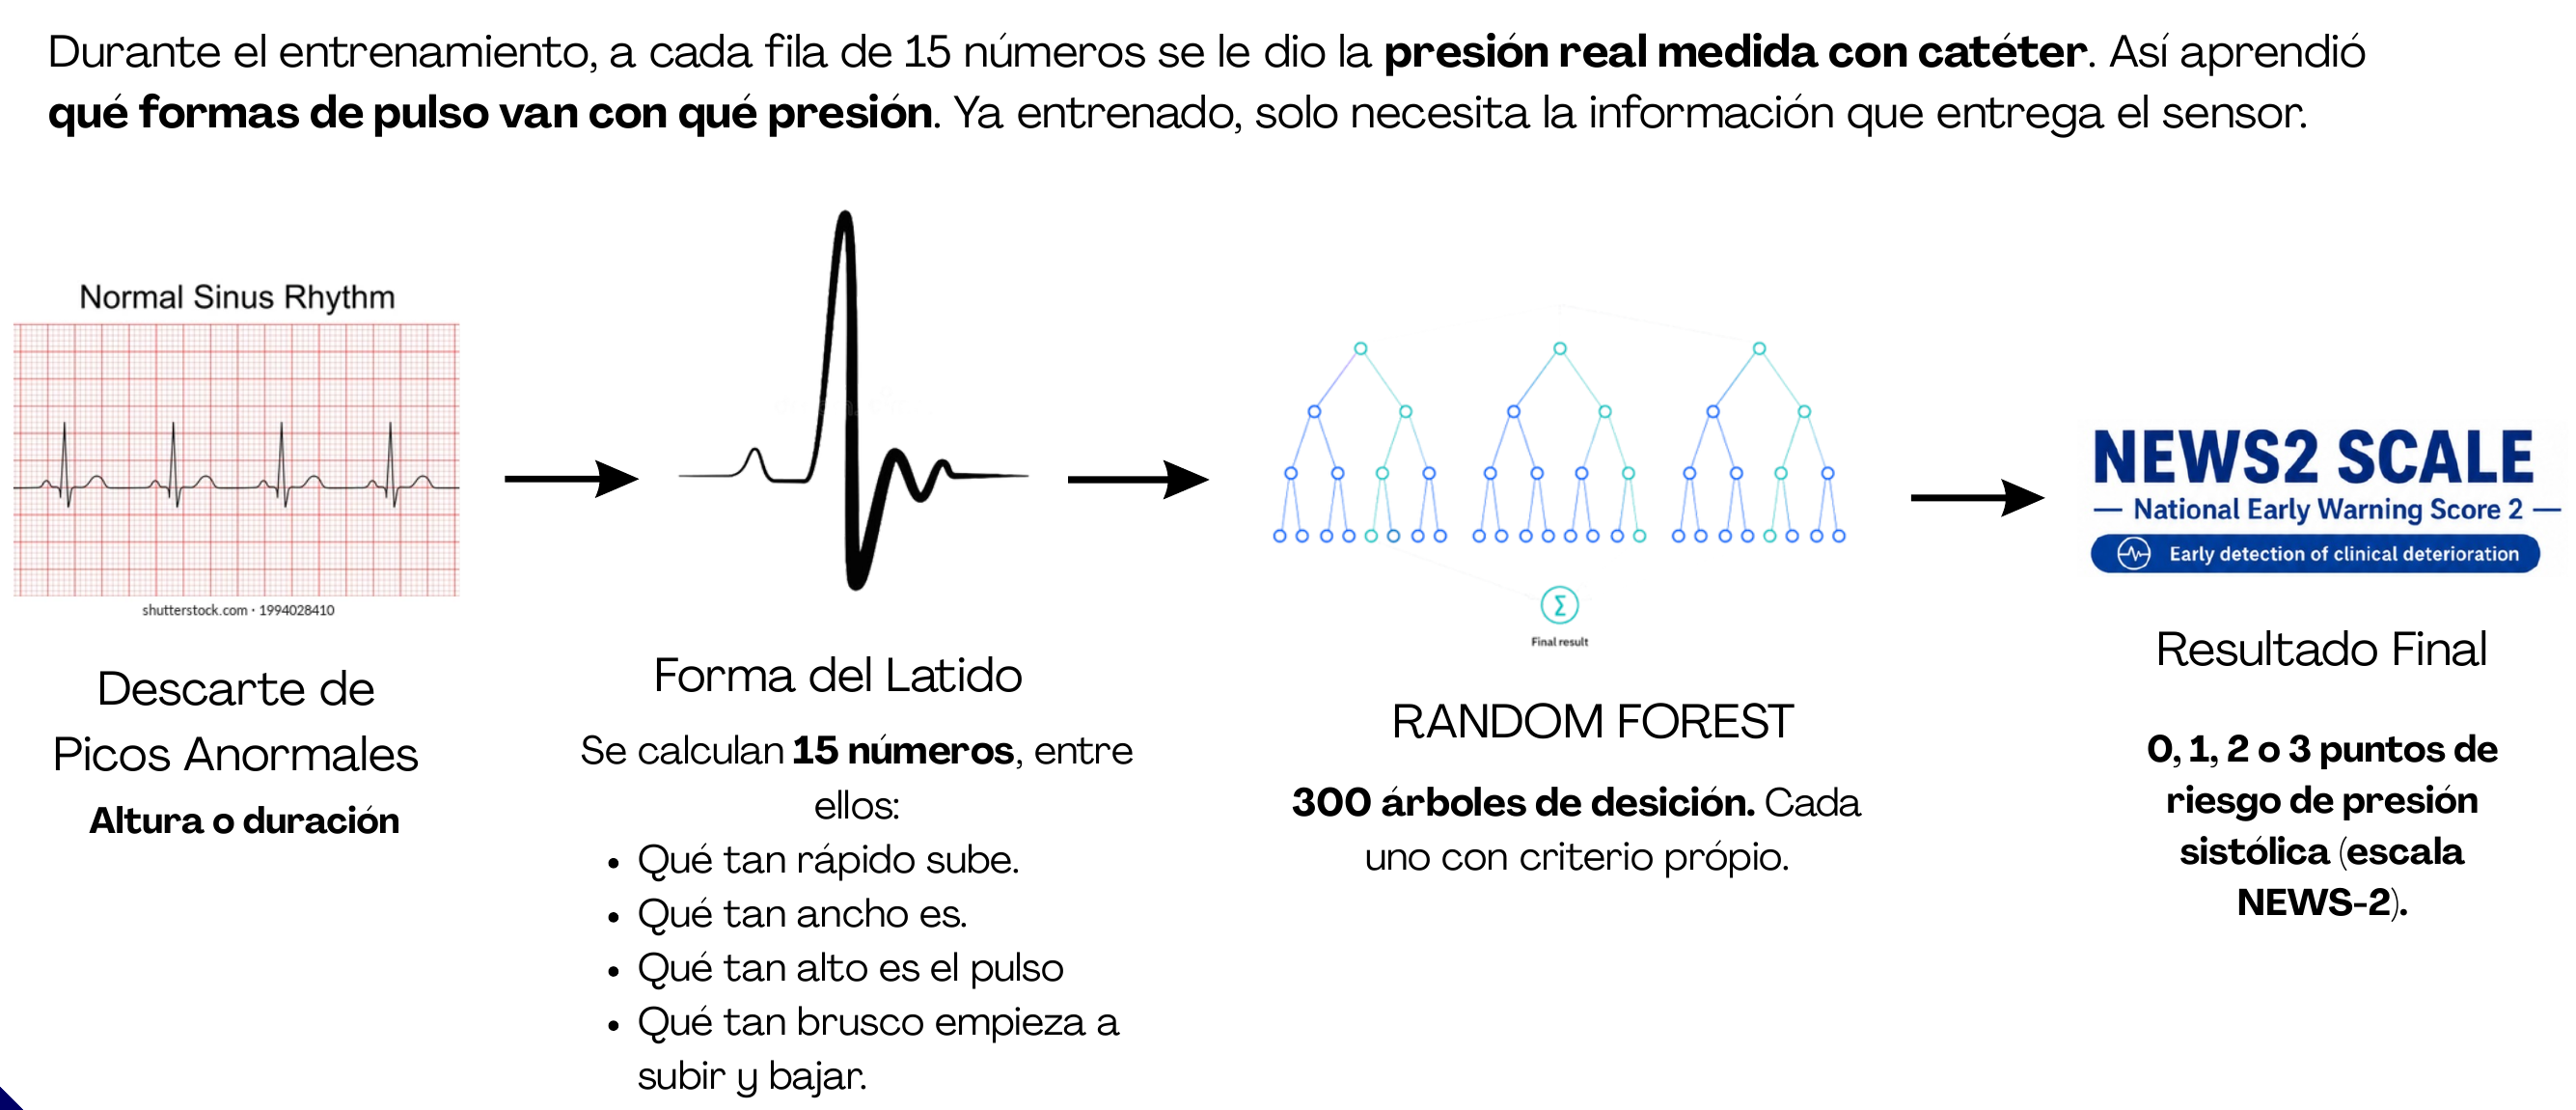
\includegraphics[width=0.95\linewidth]{modelo_rf.png}
    \caption{Funcionamiento del clasificador \textit{Random Forest} de riesgo de presión arterial.}
    \label{fig:modelo_rf}
\end{figure}

Se mantuvo el algoritmo \textit{Random Forest} por las razones que motivaron su elección al comienzo del proyecto: costo computacional adecuado para la Raspberry Pi 3, inferencia sin GPU y bajo requerimiento de ajuste de hiperparámetros. La configuración utilizada fue la siguiente:

\begin{itemize}
    \item 300 árboles de decisión, sin límite de profundidad y con un mínimo de 10 muestras por hoja, lo cual evita que los árboles memoricen ventanas individuales.
    \item Peso balanceado por clase, donde cada clase $c$ recibe un peso inversamente proporcional a su frecuencia:
    \begin{equation}
        w_c = \frac{N}{K \cdot N_c}
    \end{equation}
    siendo $N$ el número total de ventanas, $K=4$ el número de clases y $N_c$ el número de ventanas de la clase $c$. Dado que la mayoría de los datos corresponde a presiones normales, sin este ajuste el modelo tendería a predecir siempre la clase mayoritaria; con él, un error en un caso de riesgo (clase minoritaria) penaliza más que un error en un caso normal.
    \item Separación 80/20 por registro mediante \textit{GroupShuffleSplit} para la evaluación del modelo, verificando que no exista ningún registro compartido entre los conjuntos de entrenamiento y prueba.
\end{itemize}

La escala NEWS-2 no evalúa la presión de forma aislada, sino como uno de siete parámetros cuyos puntos se suman. Un error de un punto en la presión apenas modifica el puntaje total; sin embargo, la escala establece que si cualquier parámetro individual alcanza 3 puntos se debe activar una respuesta urgente sin importar el total. Por lo tanto, el error más costoso del modelo es no detectar un caso de 3 puntos. Para priorizar esta clase se modificó la regla de decisión del clasificador:

\begin{equation}
    \hat{y} =
    \begin{cases}
        3 & \text{si } p_3 \geq \tau_3 \\
        \arg\max_{c} \; p_c & \text{en otro caso}
    \end{cases}
    \qquad \tau_3 = 0.20
\end{equation}

donde $p_c$ es la probabilidad que el modelo asigna a la clase $c$ (proporción de árboles que votan por ella). El umbral $\tau_3$ se seleccionó buscando un equilibrio entre la detección de casos severos y la cantidad de falsas alarmas de escalamiento, ya que un umbral demasiado bajo genera alertas frecuentes que terminan provocando fatiga de alarma en el personal médico. El análisis de los distintos umbrales evaluados se presenta en la sección de resultados.

Una vez validado, el modelo final se entrenó con la totalidad del \textit{dataset} y se almacenó como un archivo comprimido con \textit{joblib}, junto con un archivo de metadatos que documenta las características de entrada, la regla de decisión y el umbral utilizado.

\subsubsection{Inferencia en tiempo real en la Raspberry Pi}

En la Raspberry Pi el modelo solo se carga y se utiliza para realizar predicciones; el entrenamiento se realiza fuera de línea. La inferencia se ejecuta en un hilo independiente al de lectura de los sensores, de manera que el cálculo no interrumpe la lectura de la FIFO del MAX30100. Cada 10 segundos se realiza el siguiente proceso, resumido en la Figura \ref{fig:flujo_clasificador}:

\begin{enumerate}
    \item Se toma una copia de los últimos 60 segundos de la señal IR cruda (6,000 muestras a 100~Hz). Si aún no se dispone de al menos 20 segundos de señal, no se realiza la estimación.
    \item Se aplica el mismo filtrado, detección de ciclos y extracción de características utilizados en el entrenamiento, ajustando la frecuencia de muestreo a la del MAX30100.
    \item Debido a que la señal del MAX30100 se expresa en unidades del conversor analógico-digital y la del \textit{dataset} está normalizada, se reescala la amplitud de la señal filtrada para llevarla a la escala de entrenamiento:
    \begin{equation}
        x' = x \cdot \frac{A_{ref}}{P_{95}(x) - P_{5}(x)}, \qquad A_{ref} = 1.76
    \end{equation}
    donde $P_{95}$ y $P_{5}$ son los percentiles 95 y 5 de la señal y $A_{ref}$ es la amplitud típica del \textit{dataset} de entrenamiento.
    \item Si se detectan al menos 10 ciclos válidos, se calcula la mediana de las características de los últimos 10 ciclos, igual que en las ventanas de entrenamiento, y se obtienen los puntos NEWS-2 de presión con la regla de decisión descrita. En caso contrario el valor se reporta como no disponible.
\end{enumerate}

\begin{figure}[H]
\centering
\begin{tikzpicture}[
    node distance=0.45cm,
    box/.style={draw, rounded corners, align=center, text width=11cm, minimum height=0.8cm, font=\small, fill=blue!6},
    arr/.style={-{Stealth}, thick}
]
\node[box] (a) {Buffer de señal IR cruda del MAX30100 (últimos 60 s, 100 Hz)};
\node[box, below=of a] (b) {Filtro pasa-banda Butterworth 0.5--8 Hz + reescalado de amplitud};
\node[box, below=of b] (c) {Detección de ciclos (inicio, pico sistólico, siguiente inicio) y filtros de calidad};
\node[box, below=of c] (d) {Extracción de 15 características por ciclo y mediana de los últimos 10 ciclos};
\node[box, below=of d] (e) {Random Forest Classifier (300 árboles) $\rightarrow$ probabilidades $p_0, p_1, p_2, p_3$};
\node[box, below=of e] (f) {Regla de decisión: $\hat{y}=3$ si $p_3 \geq 0.20$, si no $\arg\max p_c$};
\node[box, below=of f, fill=orange!10] (g) {Puntos NEWS-2 de presión $\rightarrow$ cálculo del NEWS-2 total $\rightarrow$ SenML / ThingSpeak};
\draw[arr] (a) -- (b);
\draw[arr] (b) -- (c);
\draw[arr] (c) -- (d);
\draw[arr] (d) -- (e);
\draw[arr] (e) -- (f);
\draw[arr] (f) -- (g);
\end{tikzpicture}
\caption{Flujo de inferencia del clasificador de riesgo de presión arterial en la Raspberry Pi.}
\label{fig:flujo_clasificador}
\end{figure}

\subsubsection{Cálculo del puntaje NEWS-2}

Con los puntos de presión obtenidos por el clasificador y los puntos de frecuencia cardíaca, SpO\textsubscript{2}, temperatura y frecuencia respiratoria, calculados con los rangos de la escala NEWS-2 \cite{ref26}, se obtiene el puntaje total como la suma de los puntos de cada parámetro. El nivel de riesgo se asigna de la siguiente manera:

\begin{itemize}
    \item \textbf{Riesgo alto:} puntaje total mayor o igual a 7, respuesta de emergencia.
    \item \textbf{Riesgo medio:} puntaje total entre 5 y 6, respuesta urgente.
    \item \textbf{Riesgo bajo-medio:} puntaje total menor a 5, pero algún parámetro individual alcanza 3 puntos, lo cual también exige una respuesta urgente.
    \item \textbf{Riesgo bajo:} puntaje total entre 1 y 4 sin parámetros en 3 puntos, vigilar.
    \item \textbf{Normal:} puntaje total igual a 0.
\end{itemize}

Los niveles se evalúan en ese orden, de modo que un puntaje total de 7 o más se clasifica como riesgo alto aunque además exista un parámetro en 3 puntos.

Los parámetros de oxigenoterapia y nivel de consciencia no pueden obtenerse con los sensores del nodo, por lo que en esta versión se asumen como paciente sin oxígeno suplementario y alerta. Si algún sensor no entrega lectura válida (por ejemplo, el dedo no está sobre el MAX30100), ese parámetro se excluye del cálculo en lugar de asumirse como normal.

\subsubsection{Presentación de los resultados en la aplicación}

Dado que el modelo no estima un valor en mmHg, la aplicación presenta la presión arterial como una categoría de riesgo, de forma consistente con las demás tarjetas de signos vitales: 0 puntos corresponde a \textit{Normal} (verde), 1 punto a \textit{Riesgo bajo} (amarillo), 2 puntos a \textit{Riesgo medio} (naranja) y 3 puntos a \textit{Riesgo alto} (rojo). La aplicación genera una alerta crítica cuando algún parámetro individual alcanza 3 puntos o cuando el puntaje NEWS-2 total es mayor o igual a 7, indicando al personal médico la causa que la originó.

\subsubsection{Interfaz de la aplicación móvil}

La aplicación cuenta con cinco pantallas (Figuras \ref{fig:app1} y \ref{fig:app2}). En la pantalla de inicio de sesión el personal médico ingresa con su correo y contraseña, y desde ella puede acceder a la creación de cuenta, donde registra su nombre, correo, contraseña y foto de perfil (tomada con la cámara o elegida de la galería). La contraseña debe tener al menos 6 caracteres, una letra mayúscula y un carácter especial. La pantalla principal saluda al usuario, muestra el estado actual del paciente con su puntaje NEWS-2, la tarjeta del nodo con su nivel de riesgo y estado de conexión, y la gráfica del histórico NEWS-2. La pantalla de detalle presenta las tarjetas de cada signo vital con su valor, su categoría de riesgo y el tiempo transcurrido desde su última actualización, incluida la presión arterial sistólica como categoría. Finalmente, la pantalla de perfil muestra los datos del usuario, el número de pacientes a cargo y el histórico de detecciones, y permite cerrar sesión.

\begin{figure}[H]
    \centering
    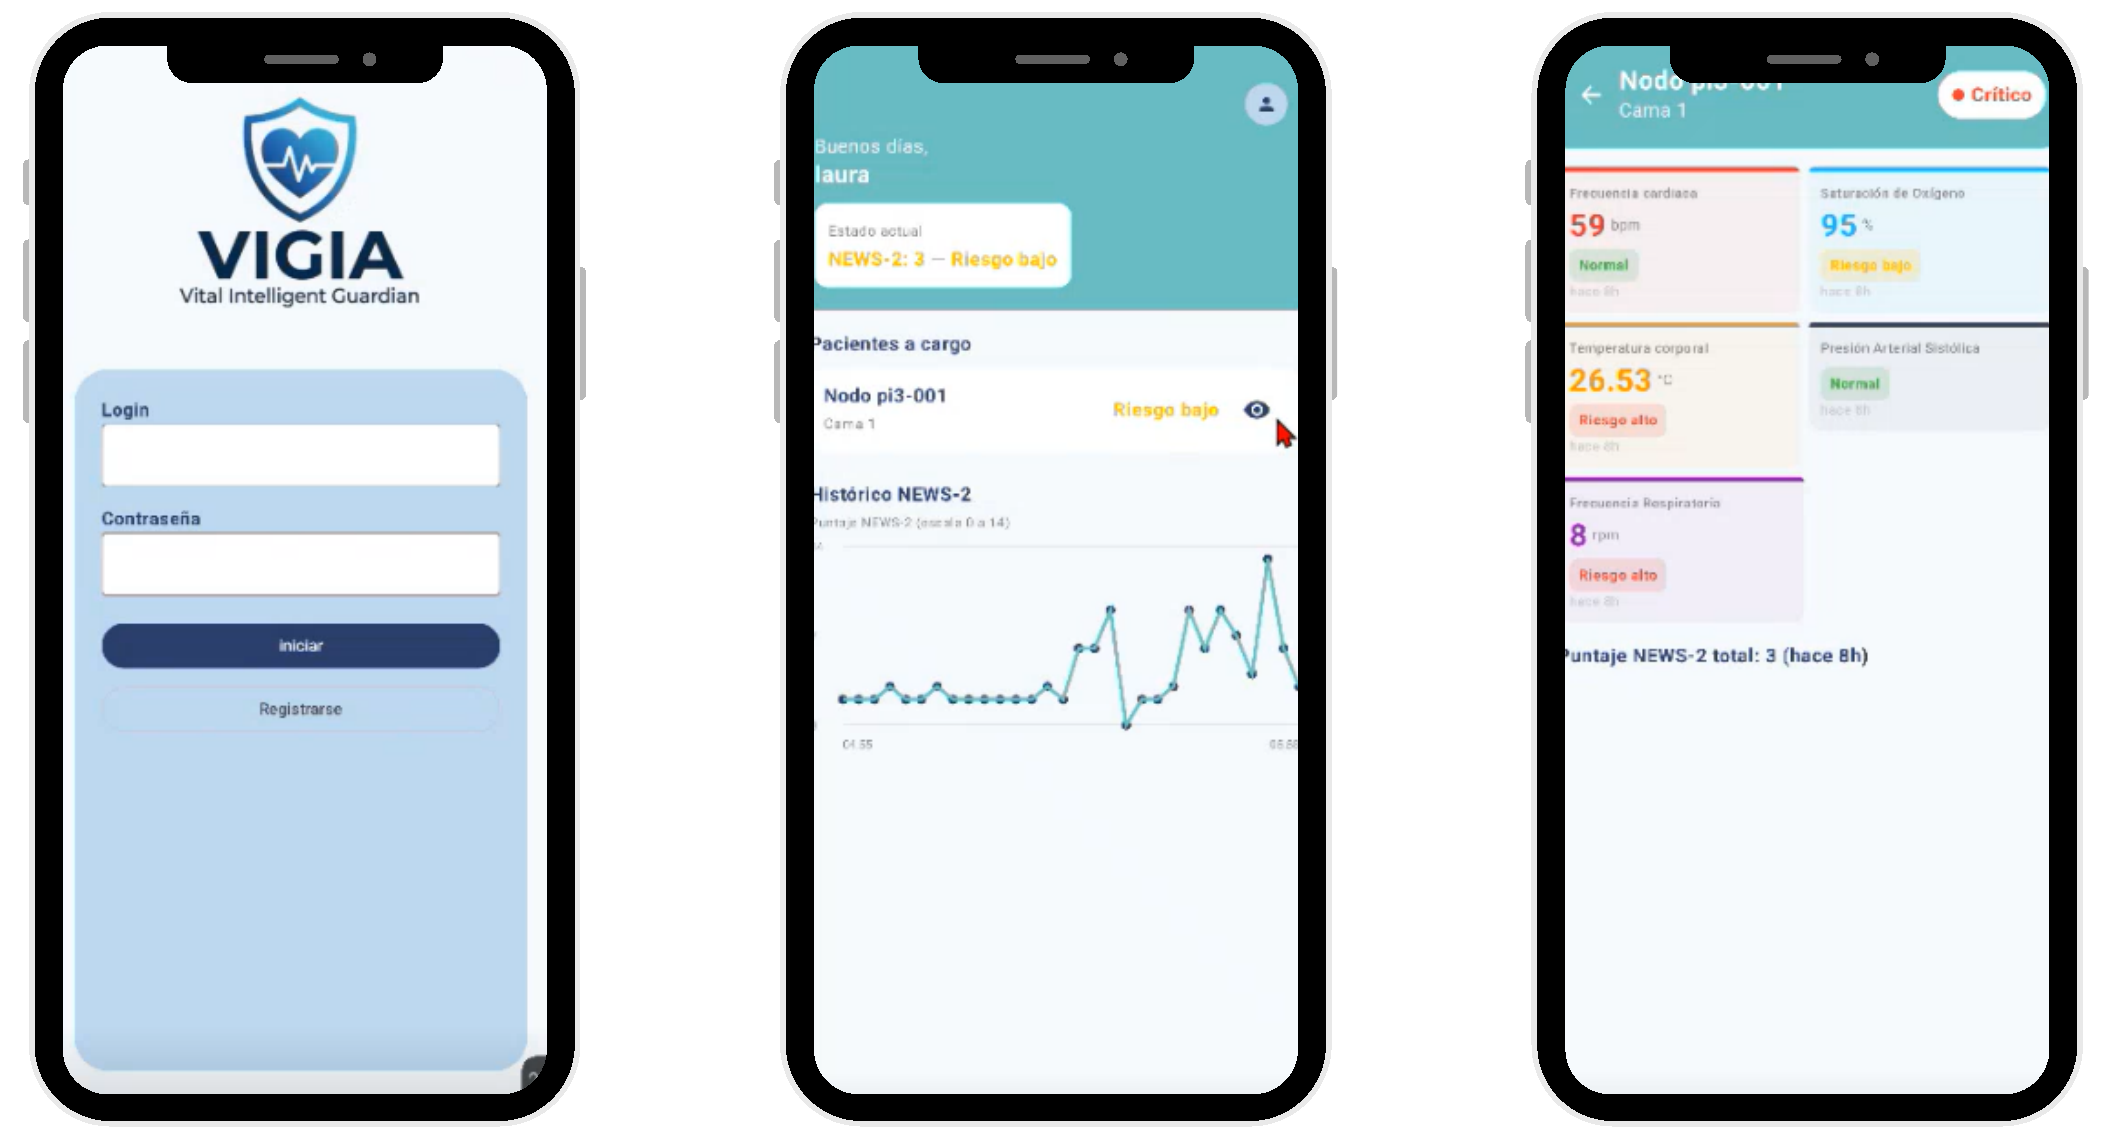
\includegraphics[width=0.85\linewidth]{app_pantallas_1.png}
    \caption{Pantallas de inicio de sesión, principal y detalle del paciente.}
    \label{fig:app1}
\end{figure}

\begin{figure}[H]
    \centering
    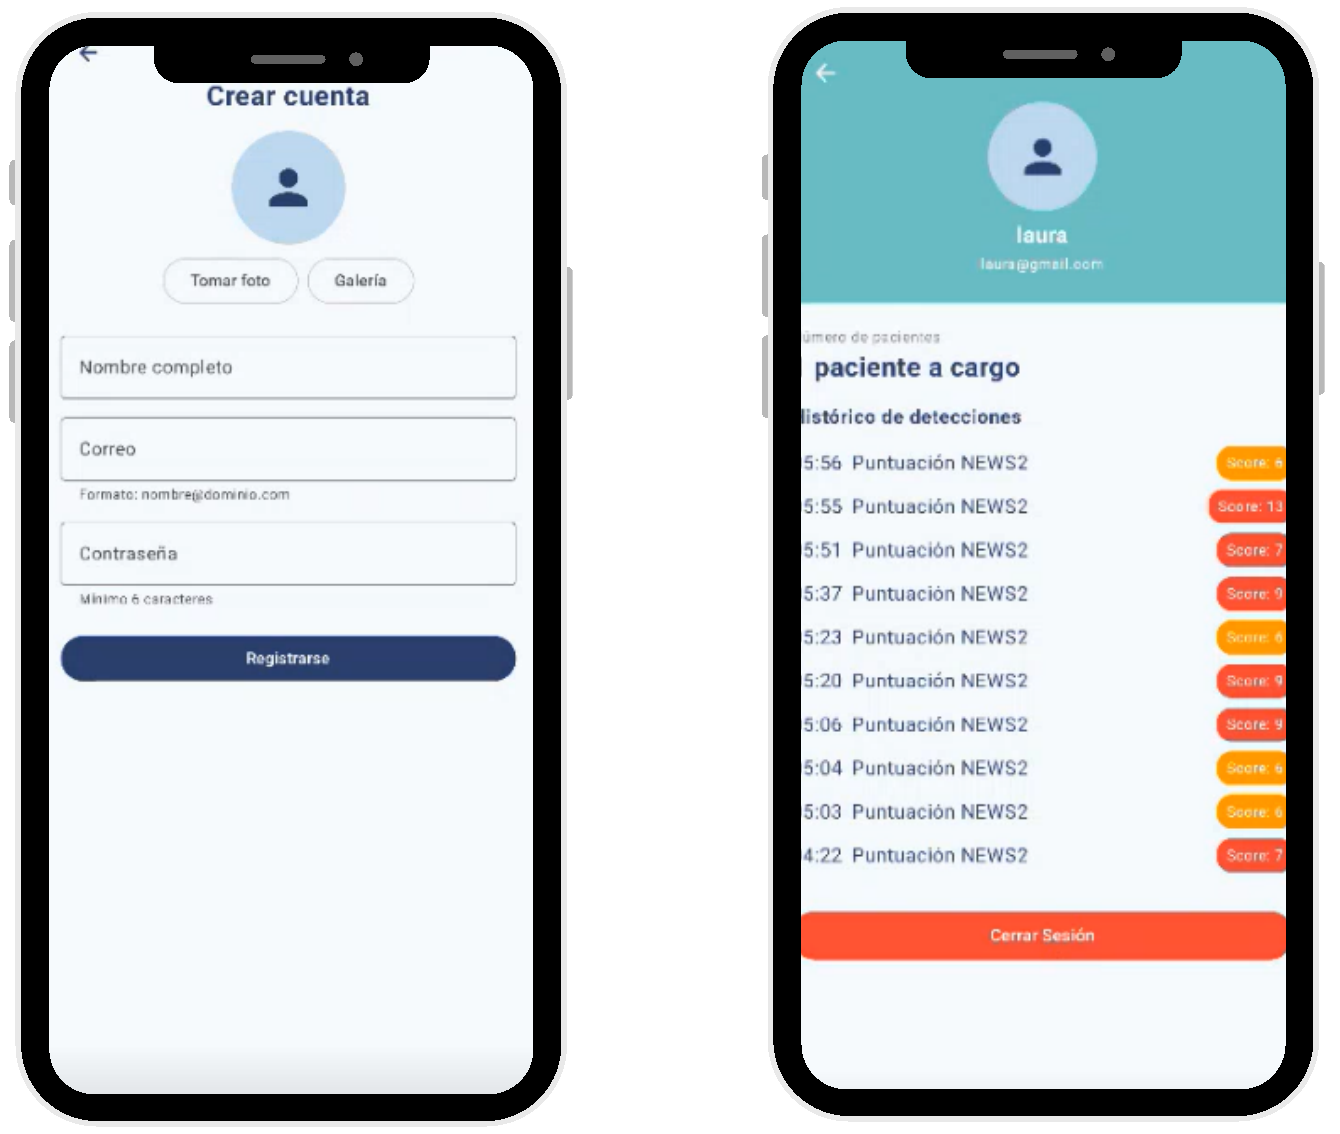
\includegraphics[width=0.55\linewidth]{app_pantallas_2.png}
    \caption{Pantallas de creación de cuenta y perfil con histórico de detecciones.}
    \label{fig:app2}
\end{figure}

\subsubsection{Diseño de la aplicación móvil}

El diseño de la aplicación se documentó mediante cuatro diagramas UML que describen sus funcionalidades, su estructura interna, su comportamiento y la interacción con los demás componentes de la solución.

\paragraph{Diagrama de casos de uso.} La Figura \ref{fig:casos_uso} presenta las funcionalidades que ofrece la aplicación y los actores que intervienen. El actor principal es el personal médico, que puede iniciar sesión, registrarse con foto de perfil, ver el estado actual del paciente, ver el detalle de los signos vitales, consultar el histórico NEWS-2, gestionar su perfil y cerrar sesión. El actor secundario es el sistema Raspberry Pi/ThingSpeak, que provee los datos del paciente. Ver el estado del paciente, ver el detalle y ver el histórico incluyen la consulta de datos a ThingSpeak, y recibir la alerta crítica extiende la visualización del estado del paciente, ya que solo ocurre cuando este se encuentra en riesgo.

\begin{figure}[H]
    \centering
    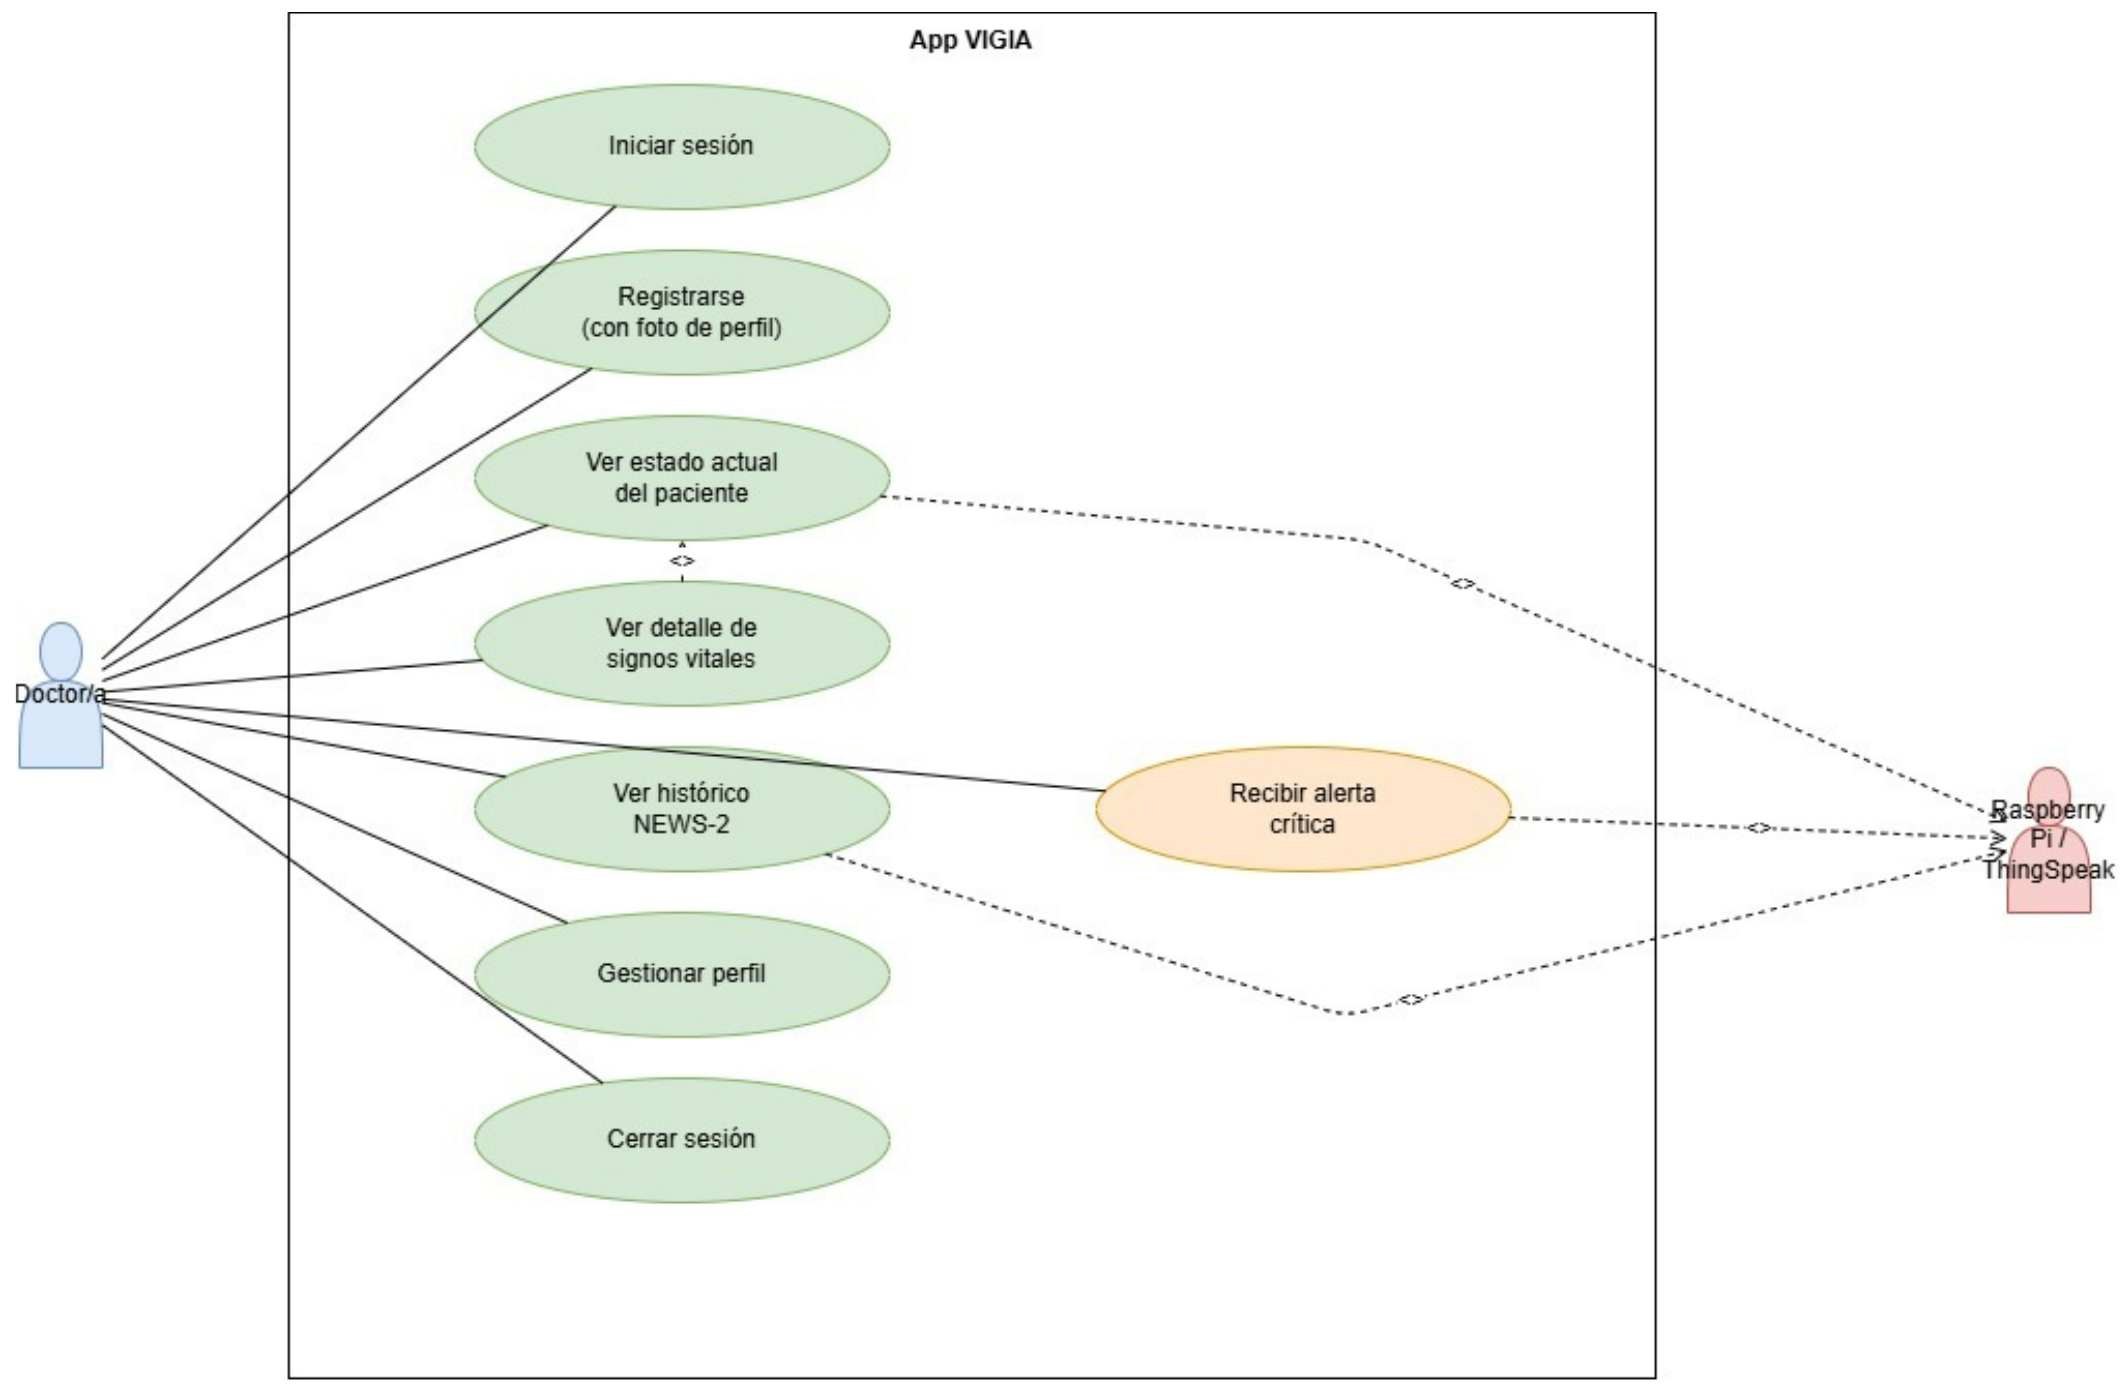
\includegraphics[width=0.8\linewidth]{caso_uso.png}
    \caption{Diagrama de casos de uso de la aplicación.}
    \label{fig:casos_uso}
\end{figure}

\paragraph{Diagrama de clases.} La Figura \ref{fig:clases} presenta la estructura interna de la aplicación. \textit{VigiaApp} es el componente raíz: controla la pantalla actual mediante la enumeración \textit{Pantalla} (LOGIN, REGISTRO, HOME, DETALLE, PERFIL), mantiene los datos más recientes del paciente y el estado de la alerta, y determina si el nodo está conectado. \textit{ThingSpeakClient} se encarga de la comunicación con la nube: obtiene la última lectura y el histórico, y crea objetos \textit{Vitales}, que almacenan el último valor de cada signo vital con su propia marca de tiempo, y \textit{AlertaHistorial}, que representa un punto del histórico NEWS-2. Las funciones de \textit{News2Utils} traducen cada signo vital a sus puntos NEWS-2 y crean la \textit{Categoria} (etiqueta y color) que se muestra en cada tarjeta.

\begin{figure}[H]
    \centering
    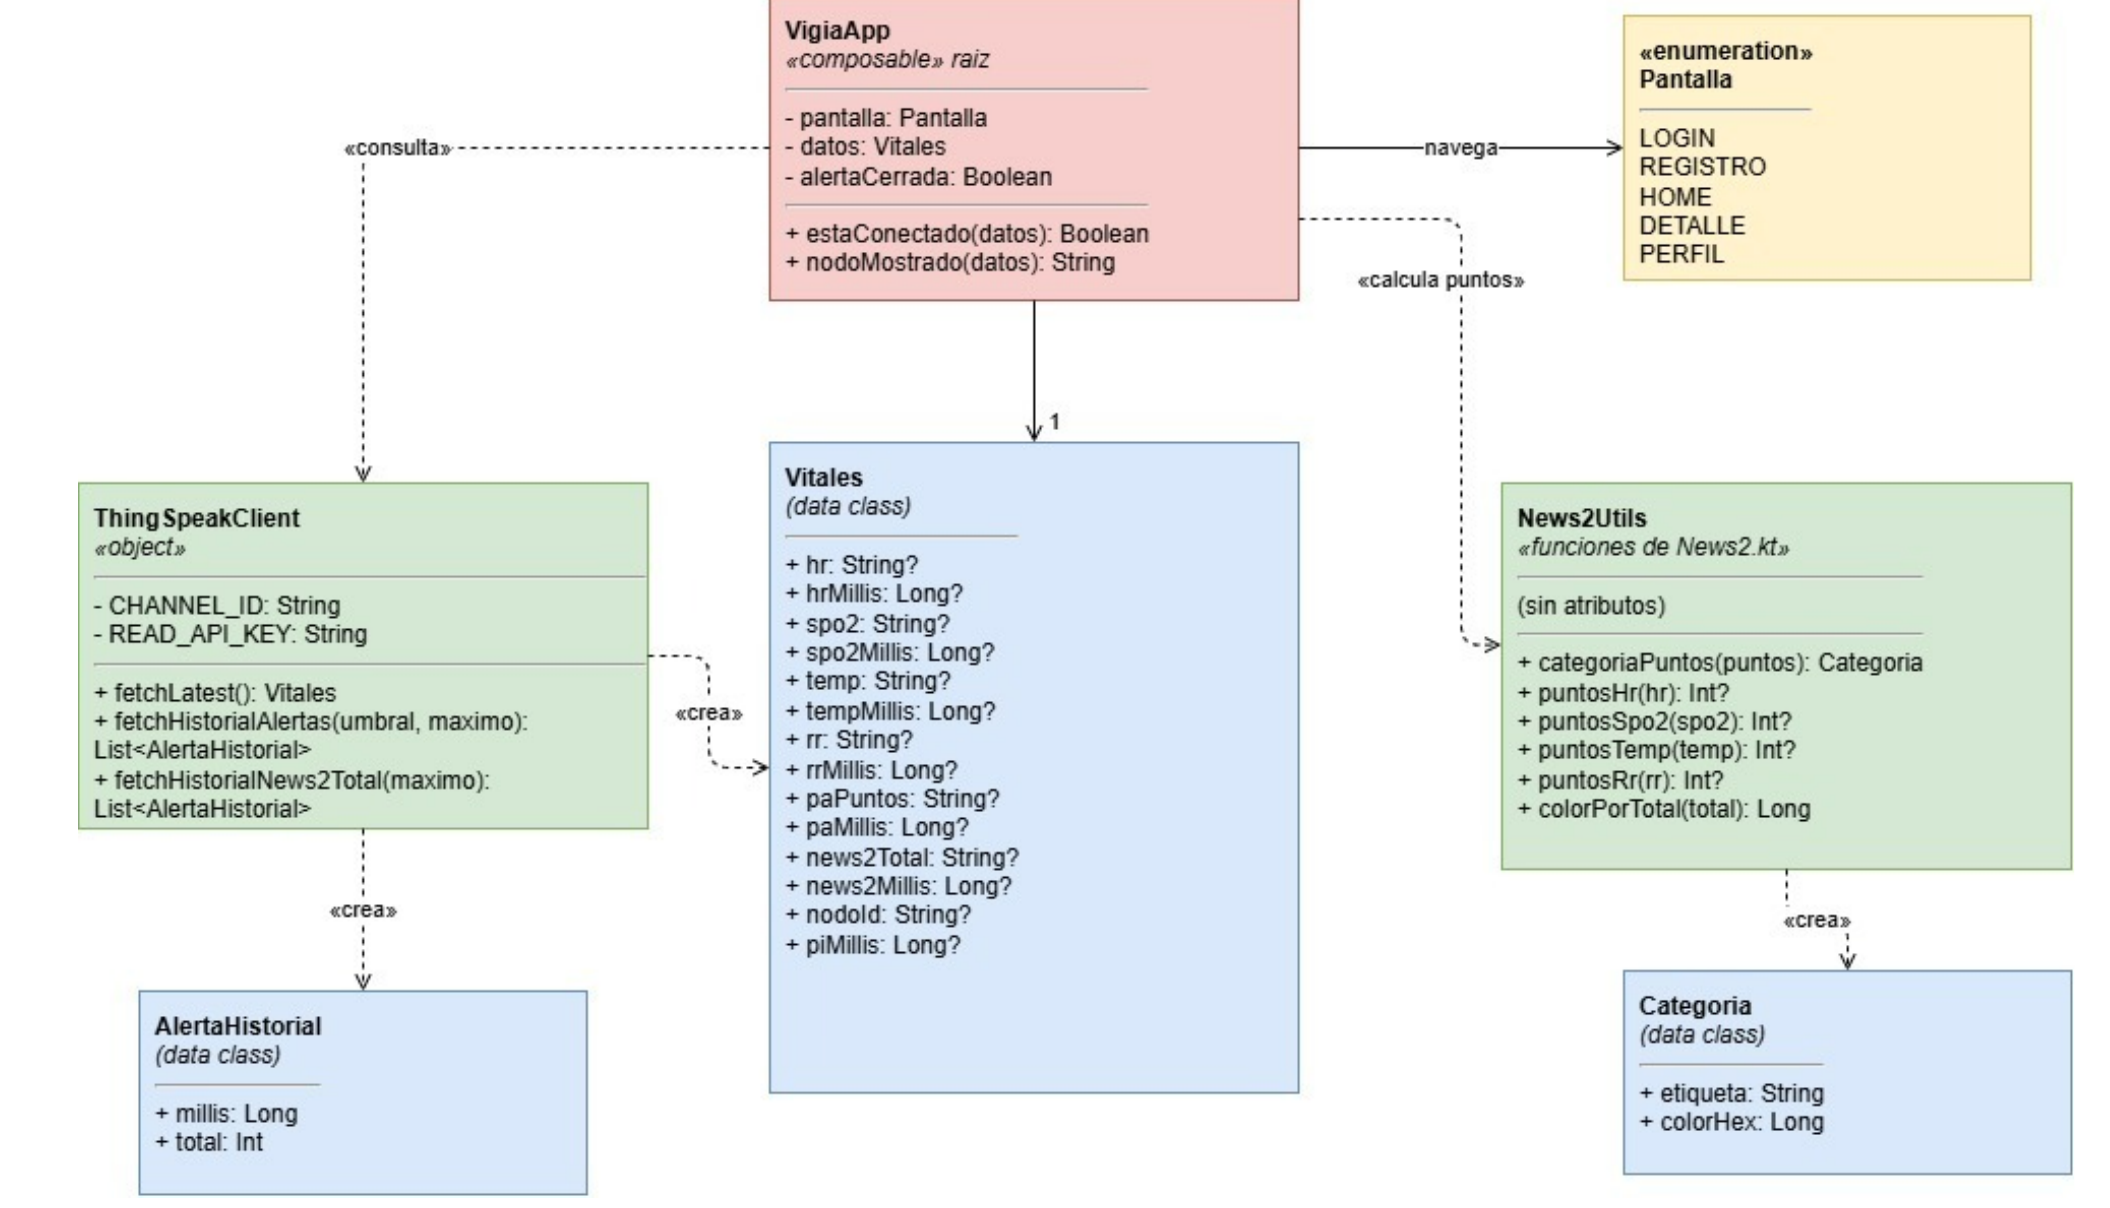
\includegraphics[width=0.9\linewidth]{clases.png}
    \caption{Diagrama de clases de la aplicación.}
    \label{fig:clases}
\end{figure}

\paragraph{Diagrama de estados.} La Figura \ref{fig:estados} describe el comportamiento de la aplicación en dos niveles. El primero corresponde a la navegación: desde LOGIN se accede a HOME tras un inicio de sesión exitoso o a REGISTRO para crear una cuenta; desde HOME se puede abrir el detalle del paciente o el perfil, y desde el perfil se cierra sesión y se regresa a LOGIN. El segundo nivel corresponde a la alerta, que funciona de forma independiente a la pantalla en la que se encuentre el usuario. En estado normal no se muestra ninguna alerta; cuando algún signo vital alcanza 3 puntos o el puntaje NEWS-2 total es mayor o igual a 7, la alerta se muestra y solo puede cerrarse presionando ACEPTAR. Mientras el paciente siga en estado crítico la alerta no se vuelve a abrir, y cuando se estabiliza la alerta se rearma para mostrarse nuevamente ante un nuevo evento crítico.

\begin{figure}[H]
    \centering
    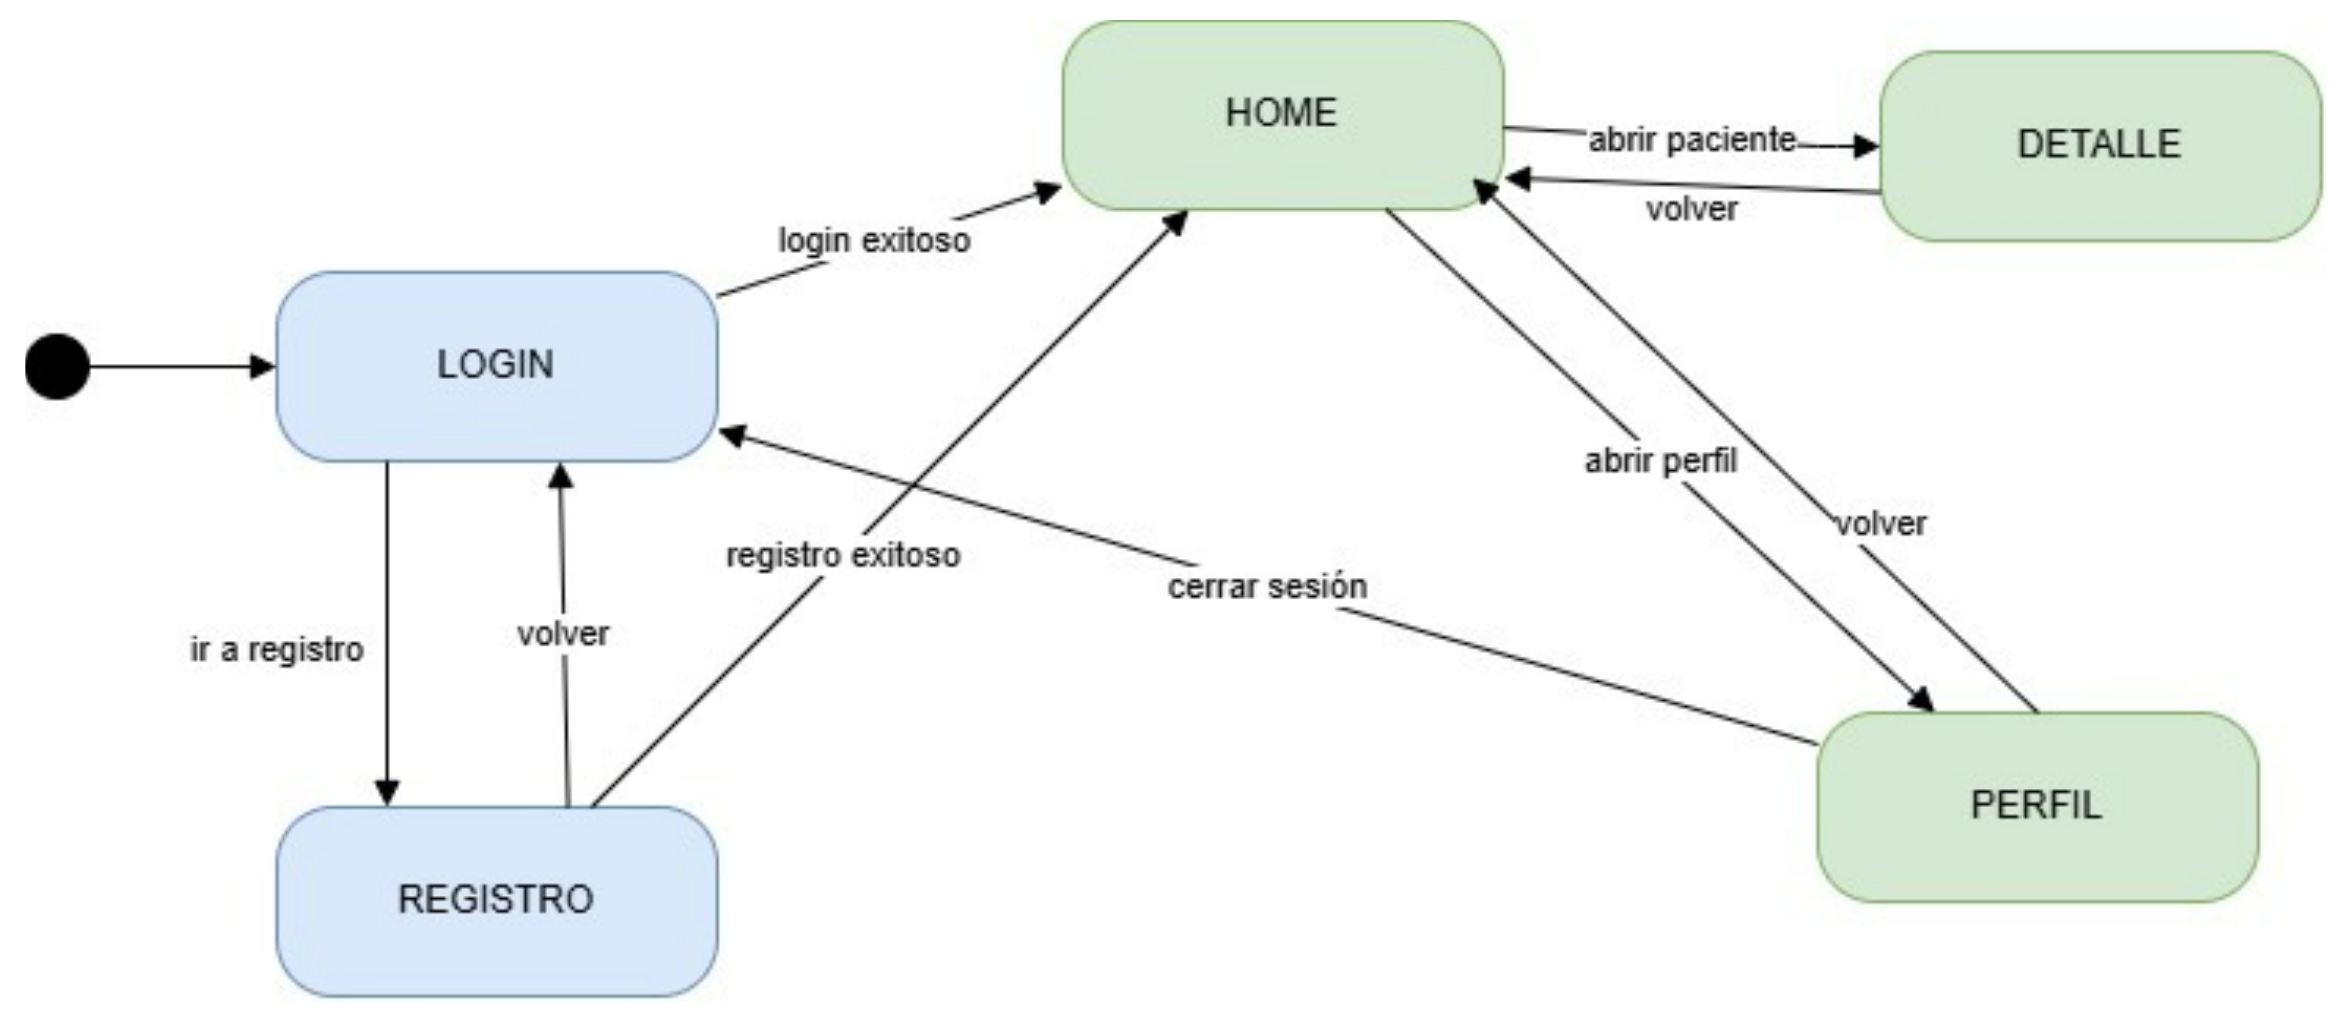
\includegraphics[width=0.85\linewidth]{estados.png}
    \caption{Diagrama de estados de la aplicación.}
    \label{fig:estados}
\end{figure}

\paragraph{Diagrama de secuencia.} La Figura \ref{fig:secuencia} describe la interacción entre los componentes de la solución durante la operación. La Raspberry Pi publica por MQTT un campo a la vez hacia ThingSpeak. En paralelo, mientras el personal médico tiene la sesión activa, la aplicación solicita cada 10 segundos las últimas 30 lecturas del canal mediante la API REST. Dado que cada mensaje contiene un solo campo, \textit{ThingSpeakClient} reconstruye el estado del paciente recorriendo las lecturas de la más reciente a la más antigua y tomando el primer valor no vacío de cada campo. Con estos datos se calculan los puntos NEWS-2 de cada signo vital y se evalúa si el paciente está en estado crítico: si lo está, se muestra la alerta crítica; en caso contrario, se actualizan las pantallas con los datos nuevos.

\begin{figure}[H]
    \centering
    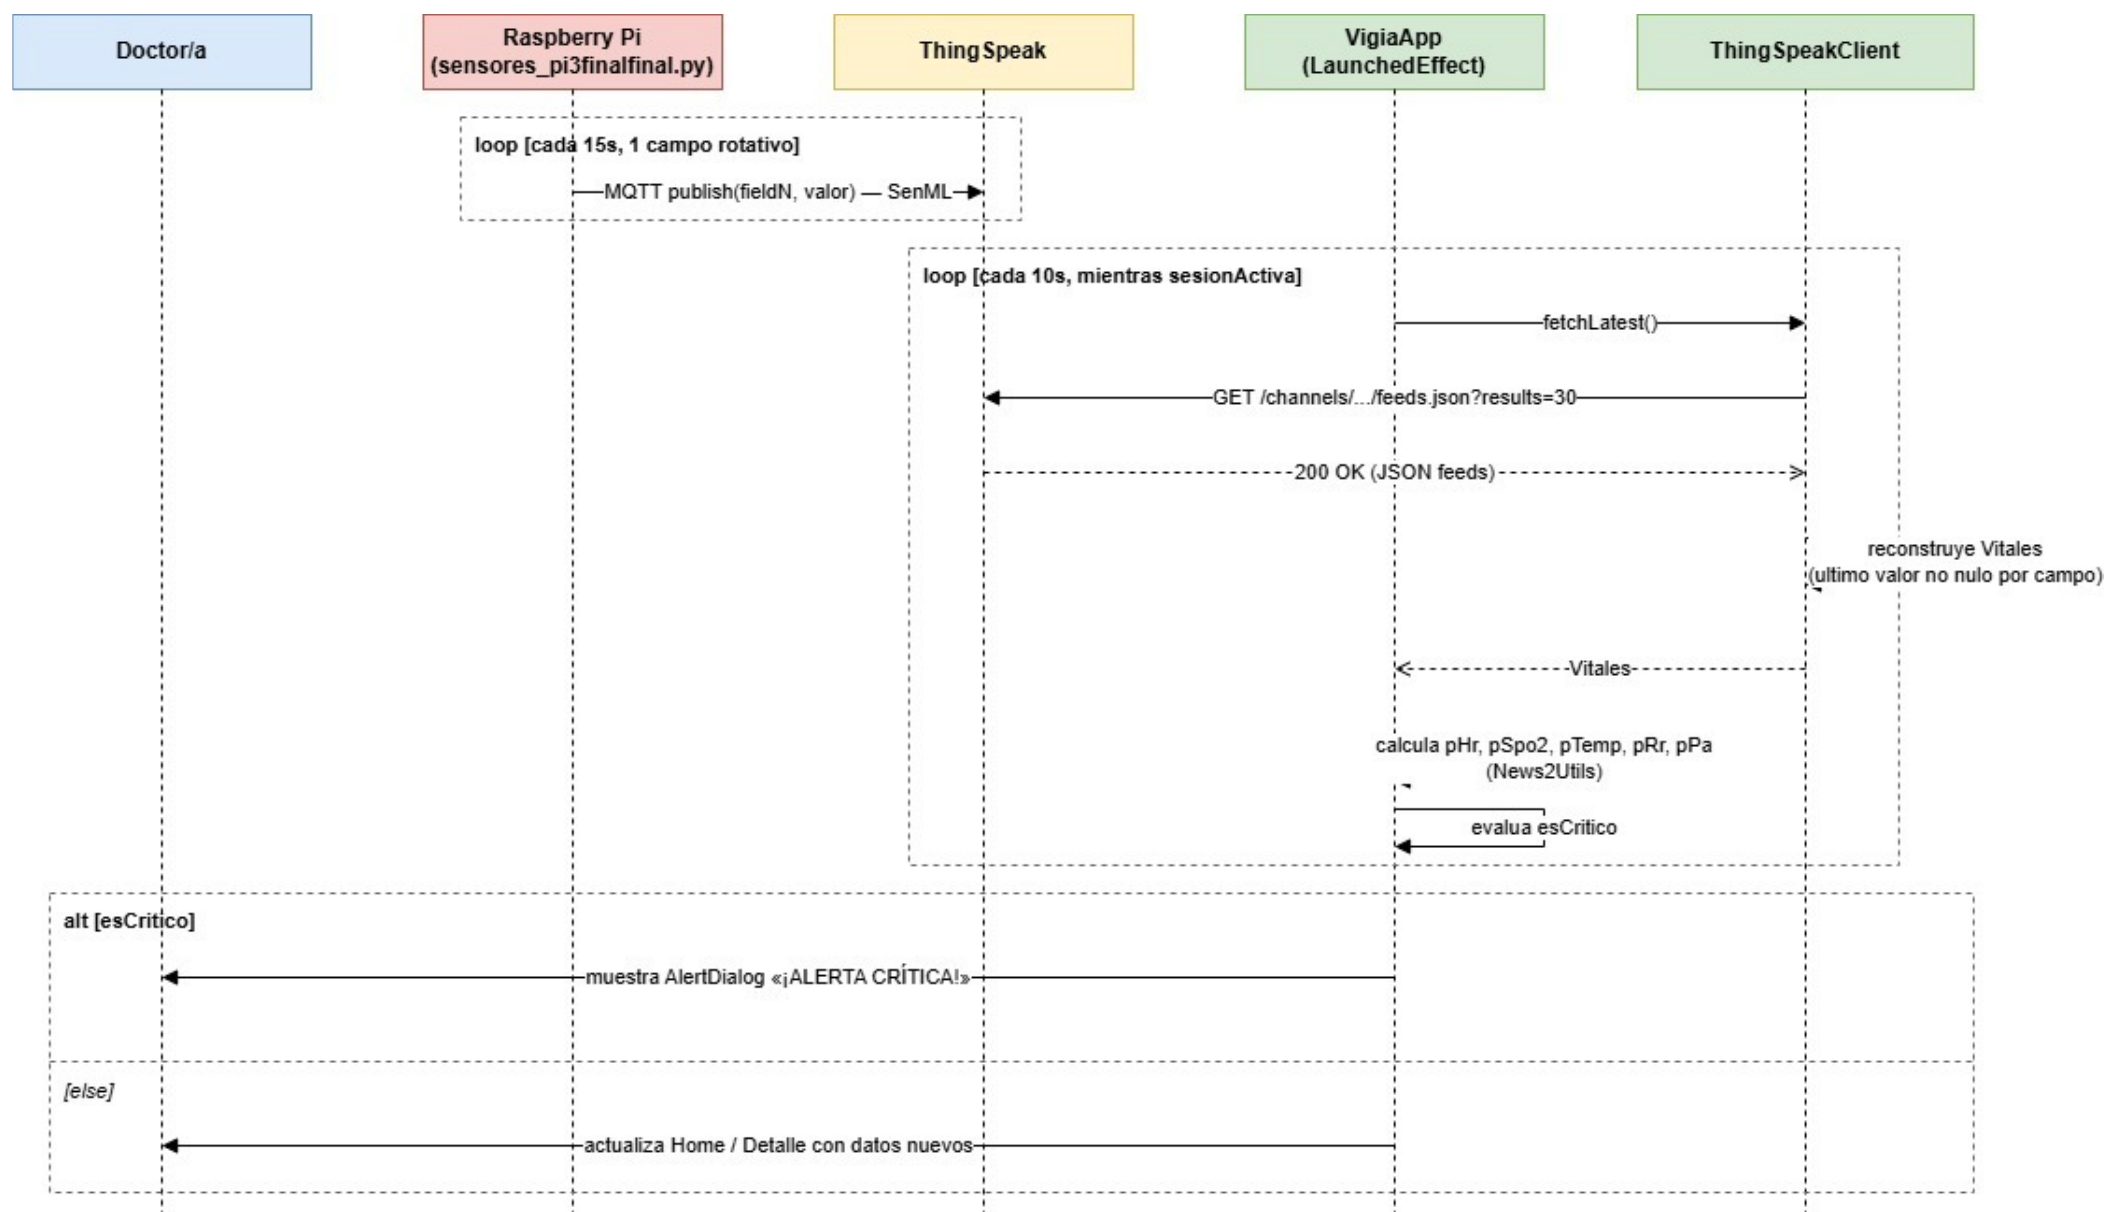
\includegraphics[width=0.9\linewidth]{secuencia.png}
    \caption{Diagrama de secuencia de la operación de la solución.}
    \label{fig:secuencia}
\end{figure}

% ------------------------------------------------------------
\section{Resultados obtenidos}\label{sec:resultados}

En esta sección se presentan los resultados del prototipo construido, las pruebas de funcionamiento del sistema completo, la interfaz web y los resultados de la analítica de datos, y se discuten los aspectos más relevantes de cada uno.

\subsection{Prototipo del nodo IoT}

sin hacer

\subsection{Pruebas de funcionamiento}

% PENDIENTE: completar la descripción de las pruebas (montaje, adquisición, transmisión y lecturas obtenidas).

\paragraph{Alerta crítica.} La Figura \ref{fig:alerta} muestra la alerta generada por la aplicación durante una de las pruebas. El nodo pi3-001 alcanzó un puntaje NEWS-2 de 8, y la aplicación indicó como causas los tres parámetros que llegaron a 3 puntos: la saturación de oxígeno (89\%), la frecuencia respiratoria (6~rpm) y la presión arterial sistólica en riesgo alto. Al fondo se observa que la pantalla principal también clasificó al paciente como \textit{Crítico}, tanto en el estado actual como en la tarjeta del nodo, y la gráfica del histórico NEWS-2 con la evolución del puntaje durante la sesión. La alerta se superpone a la pantalla en la que se encuentre el usuario y solo se cierra al presionar ACEPTAR, tal como se describió en el diagrama de estados (Figura \ref{fig:estados}).

\begin{figure}[H]
    \centering
    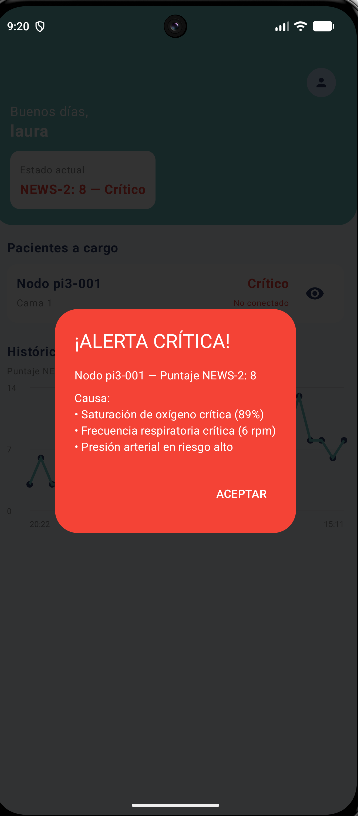
\includegraphics[width=0.35\linewidth]{captura_alerta.png}
    \caption{Alerta crítica generada por la aplicación durante las pruebas.}
    \label{fig:alerta}
\end{figure}

Las pruebas se realizaron sobre personas sanas, por lo que los valores que activaron la alerta no corresponden a un deterioro real. La SpO\textsubscript{2} de 89\% y la frecuencia respiratoria de 6~rpm reflejan la falta de calibración de estas mediciones y su sensibilidad al movimiento y al contacto del dedo con el sensor, y los 3 puntos de presión arterial son coherentes con la tasa de falsos casos de 3 puntos del clasificador (6.1\%) y con la diferencia entre la señal del MAX30100 y las señales de monitores clínicos con las que fue entrenado. Esto muestra que la lógica de alerta funciona correctamente, pero que su confiabilidad depende de la calidad de la medición de cada sensor.

\subsection{Interfaz web}

Además de la aplicación móvil, se desarrolló una página web informativa del proyecto con HTML y CSS, publicada en GitHub Pages (\url{https://llerenix.github.io/Vigia/}). La Figura \ref{fig:web} muestra la página de inicio, que presenta el propósito de VIGIA (detección temprana de sepsis mediante inteligencia artificial y sensores biométricos) y cuenta con secciones de inicio, producto, tecnología, aplicación y equipo, además de botones para conocer el proyecto, ver un video y solicitar una demostración. La Figura \ref{fig:web_laptop} muestra la página en uso desde un computador portátil.

\begin{figure}[H]
    \centering
    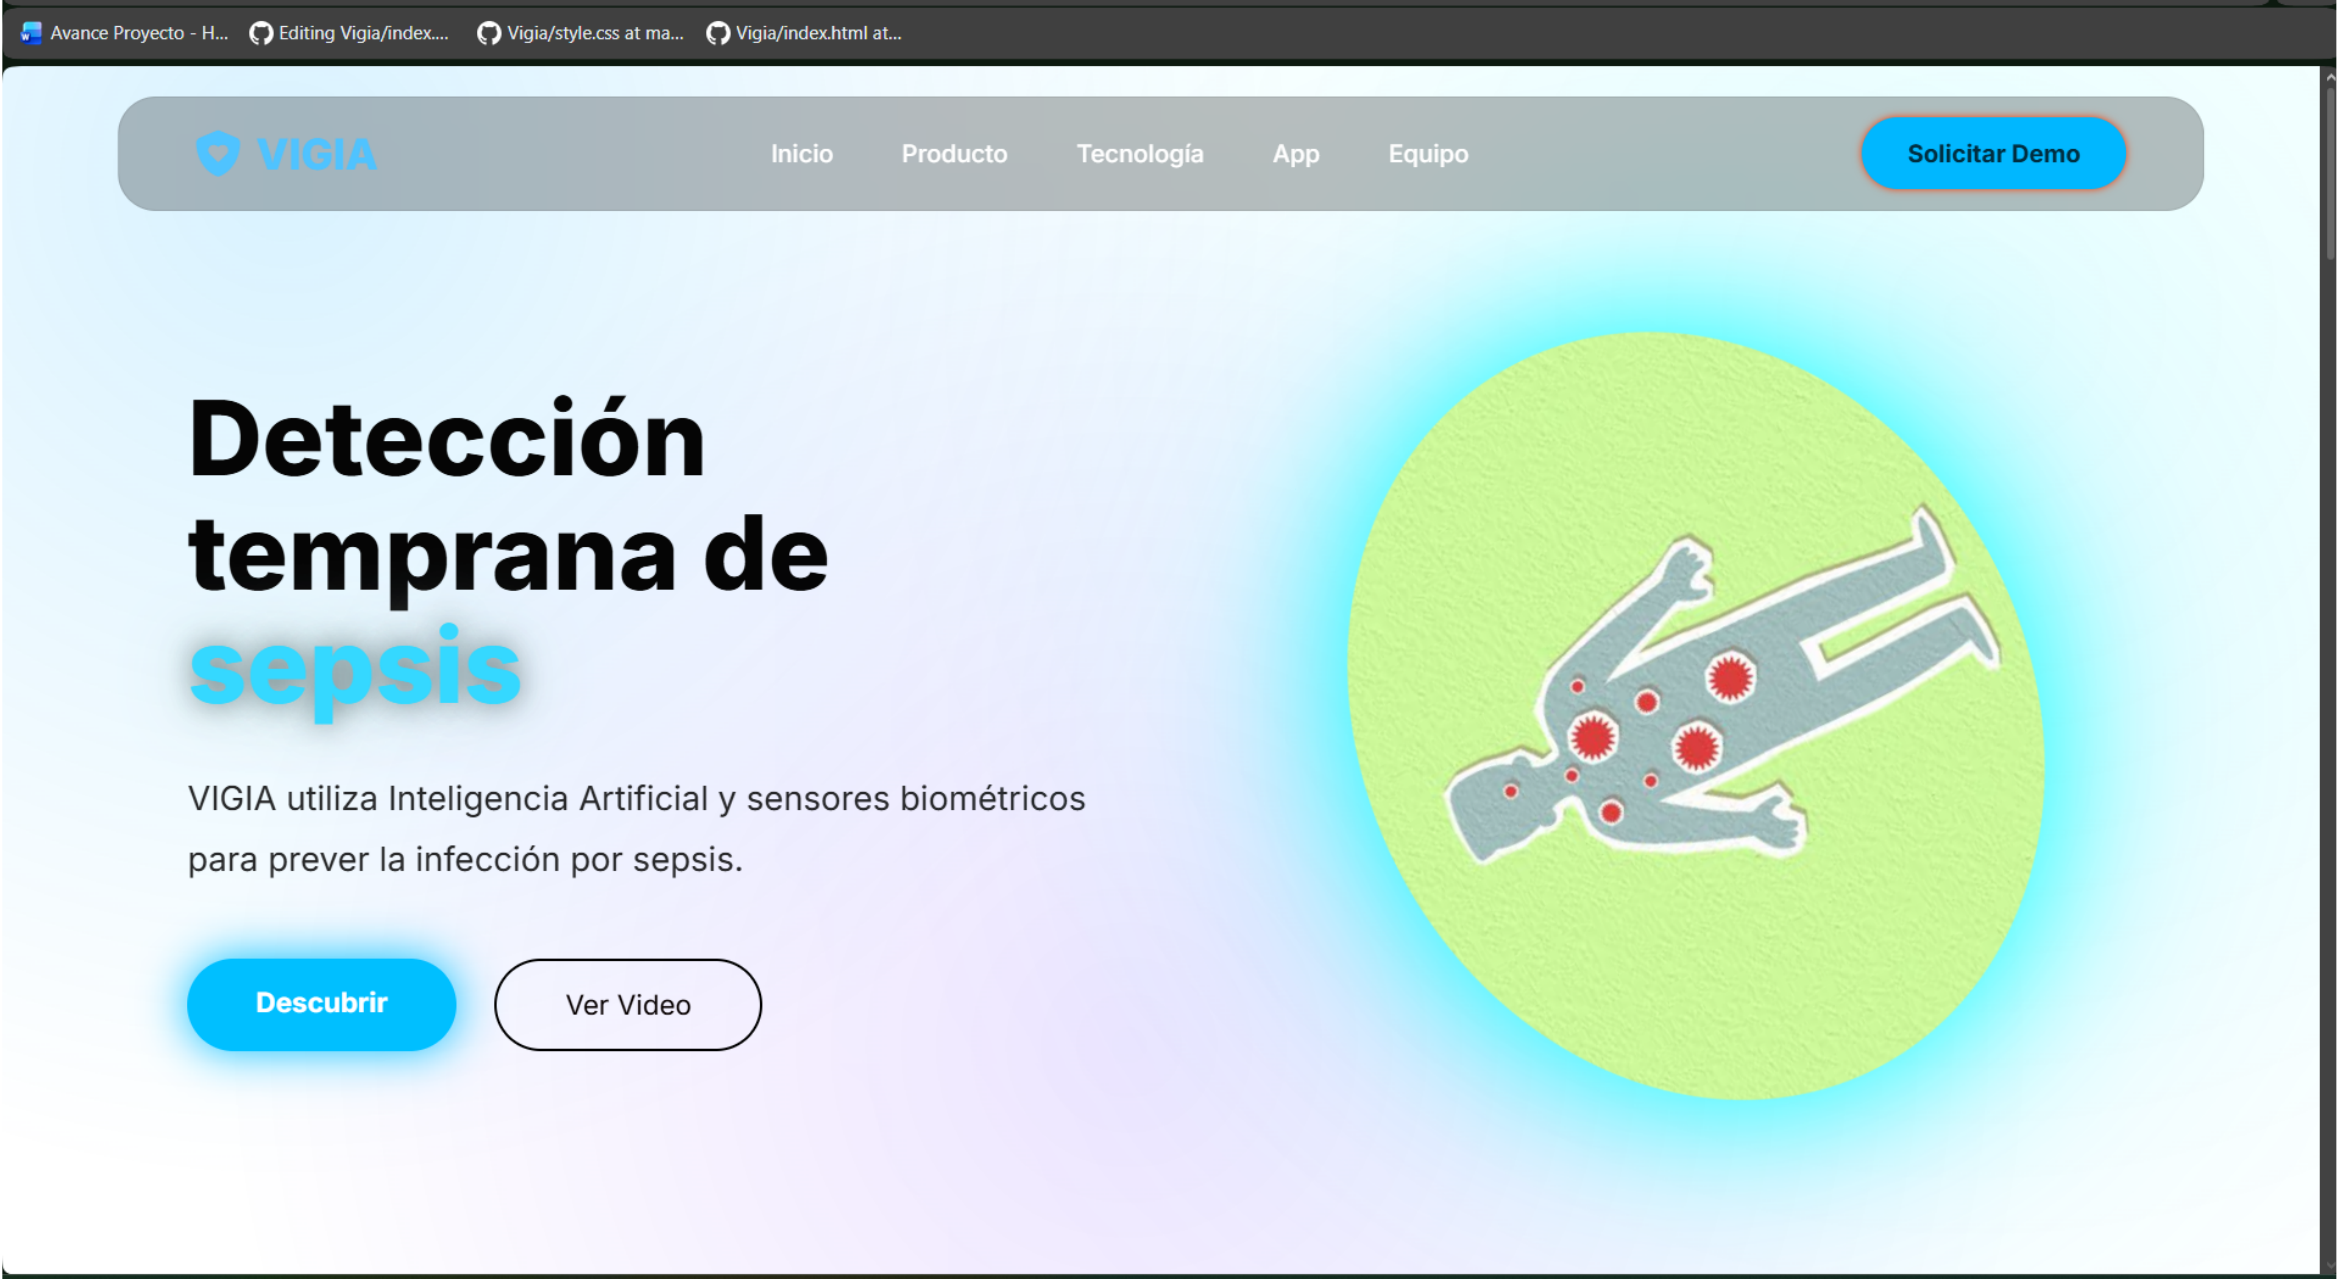
\includegraphics[width=0.85\linewidth]{web_inicio.png}
    \caption{Página de inicio de la interfaz web de VIGIA.}
    \label{fig:web}
\end{figure}

\begin{figure}[H]
    \centering
    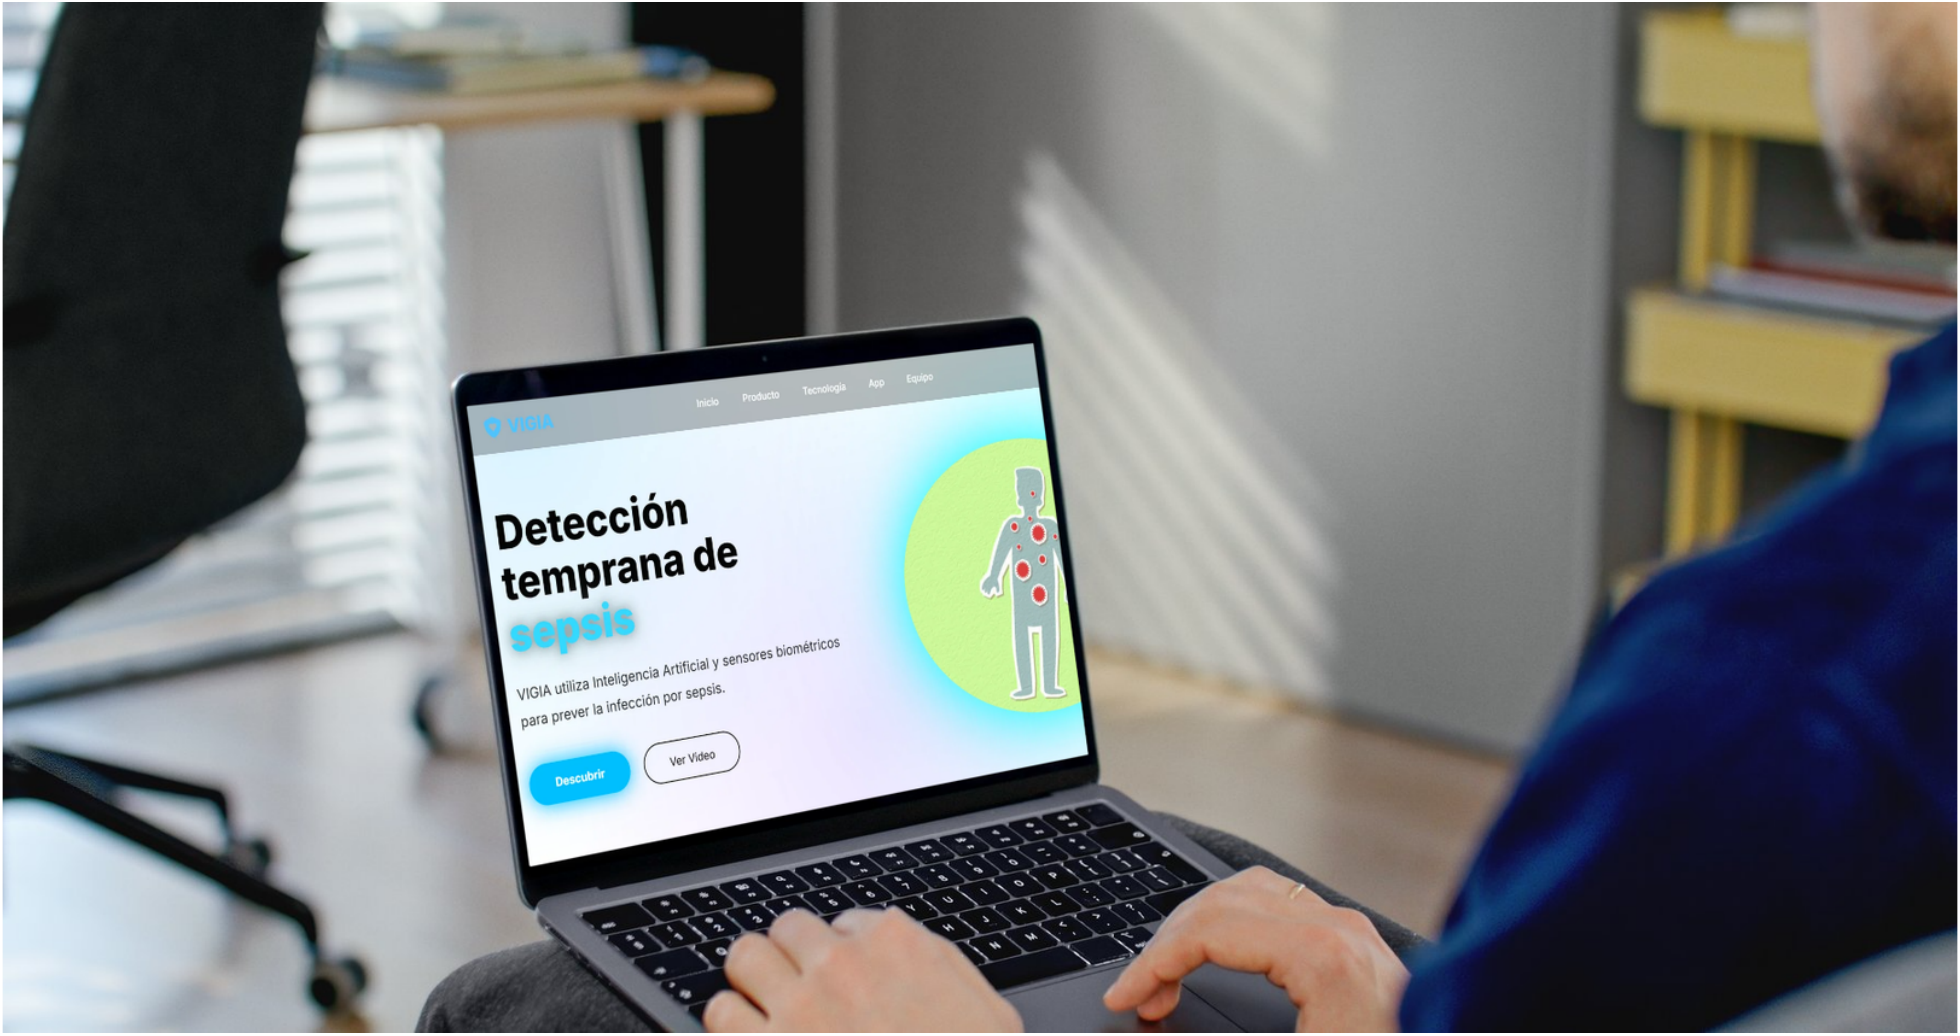
\includegraphics[width=0.7\linewidth]{web_laptop.png}
    \caption{Interfaz web de VIGIA en uso.}
    \label{fig:web_laptop}
\end{figure}

\subsection{Resultados de la analítica de datos}

\subsubsection{Distribución de los datos}

La Figura \ref{fig:dist_clases} presenta la distribución de los puntos NEWS-2 de presión sistólica en las 119,880 ventanas del \textit{dataset}. El 79.9\% de las ventanas corresponde a presiones normales (0 puntos), mientras que solo el 2.0\% corresponde a casos de 3 puntos. Este desbalance es determinante en los resultados que se presentan a continuación: un modelo que siempre predijera ``normal'' acertaría cerca del 80\% de las veces sin detectar ningún caso de riesgo, por lo que la exactitud general no es una métrica adecuada para evaluar este problema y se utilizan en su lugar la sensibilidad y la tasa de falsas alarmas.

\begin{figure}[H]
    \centering
    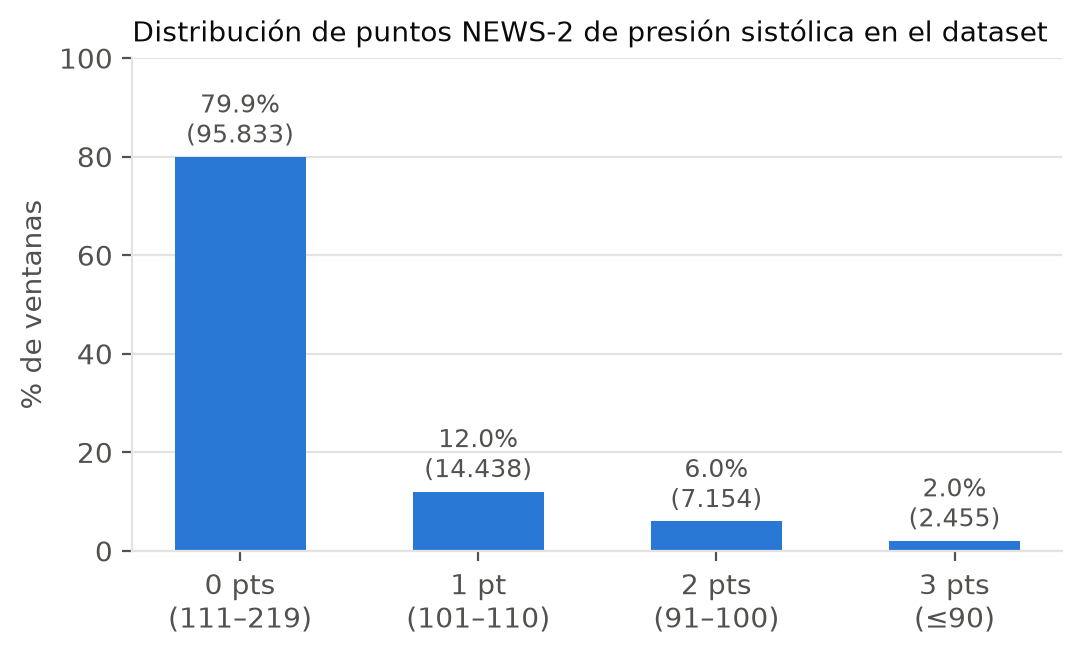
\includegraphics[width=0.7\linewidth]{res_distribucion_clases.png}
    \caption{Distribución de los puntos NEWS-2 de presión sistólica en el \textit{dataset} de entrenamiento.}
    \label{fig:dist_clases}
\end{figure}

\subsubsection{Estimación de presión en mmHg}

La Tabla \ref{tab:regresion} presenta los resultados del \textit{Random Forest Regressor} sobre el conjunto de prueba (23,957 ventanas de 2,205 registros no vistos en el entrenamiento). La primera configuración utiliza las 11 características iniciales de la Tabla \ref{tab:features}; la segunda agrega cuatro características morfológicas (\textit{area\_ratio}, \textit{notch\_depth\_ratio}, \textit{aug\_index} y \textit{spectral\_ratio}). Al agregarlas, la desviación estándar del error bajó de 17.06 a 16.68~mmHg, pero en ambos casos es más del doble del límite del estándar AAMI \cite{ref23}, por lo que el modelo no cumple el criterio clínico, aunque el sesgo sí se encuentra dentro del límite.

\begin{table}[H]
\centering
\begin{tabular}{lccc}
\toprule
\textbf{Configuración} & \textbf{MAE (mmHg)} & \textbf{Sesgo (mmHg)} & \textbf{SD del error (mmHg)} \\
\midrule
11 características & 12.97 & 0.66 & 17.06 \\
15 características & 12.66 & 0.71 & 16.68 \\
\midrule
Requisito AAMI & -- & $\leq 5$ & $\leq 8$ \\
\bottomrule
\end{tabular}
\caption{Resultados del regresor de presión sistólica en el conjunto de prueba.}
\label{tab:regresion}
\end{table}

Para determinar si el error podía reducirse se realizaron cuatro experimentos. Primero, con las 11 características iniciales, se evaluaron cinco configuraciones adicionales del modelo, desde una muy podada (3~MB) hasta una de 300 árboles sin límite de profundidad (623~MB), obteniendo MAE entre 13.29 y 14.83~mmHg; ninguna superó a la configuración de referencia de la Tabla \ref{tab:regresion} (12.97~mmHg), por lo que aumentar la capacidad no mejoró el resultado. Segundo, se construyó la curva de aprendizaje de la Figura \ref{fig:curva}: el error disminuye al aumentar los datos, pero con rendimientos decrecientes, y su extrapolación indica un techo cercano a 12.6~mmHg incluso con datos ilimitados del mismo tipo. Tercero, se entrenaron modelos especializados por grupos de pacientes (agrupamiento KMeans con 3, 5 y 8 grupos), con MAE entre 12.92 y 13.02~mmHg, sin diferencia frente al modelo único. Cuarto, la descomposición de la varianza del error mostró que el 85.2\% se debe a diferencias entre registros y solo el 14.8\% a variaciones dentro de un mismo registro; por esta razón, promediar 10 ventanas del mismo paciente solo reduce la desviación estándar de 17.06 a 15.88~mmHg.

\begin{figure}[H]
    \centering
    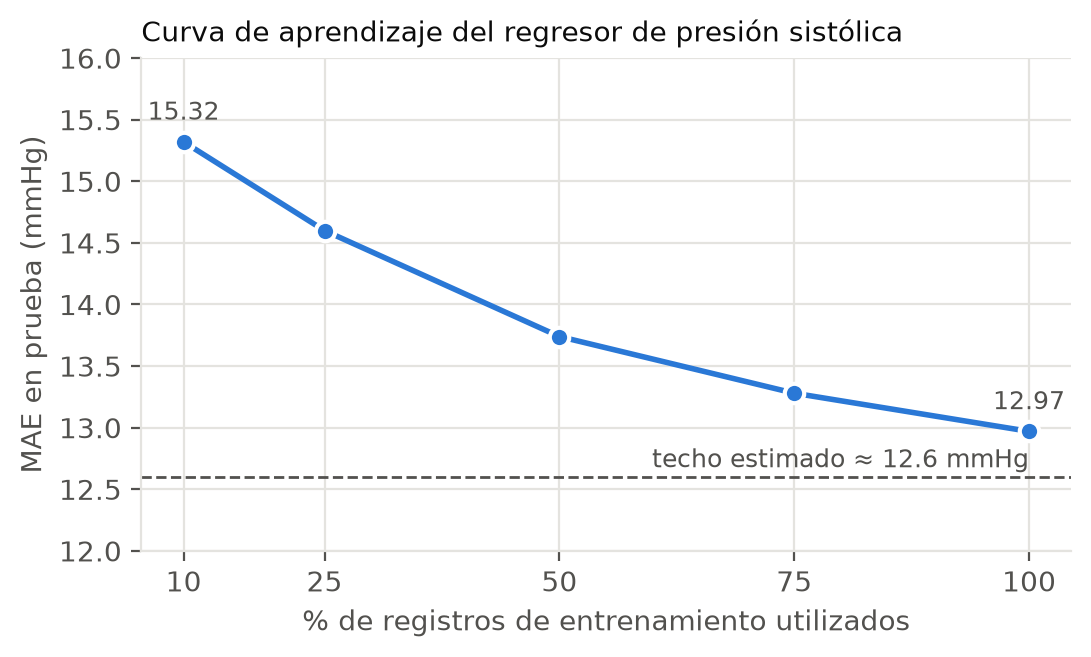
\includegraphics[width=0.7\linewidth]{res_curva_aprendizaje.png}
    \caption{Curva de aprendizaje del regresor: error absoluto medio en prueba frente a la cantidad de datos de entrenamiento.}
    \label{fig:curva}
\end{figure}

Estos resultados indican que el error no se debe a la capacidad del modelo, a la cantidad de datos ni al ruido de medición, sino a un sesgo sistemático propio de cada paciente que la señal PPG por sí sola no permite corregir. La Tabla \ref{tab:literatura} compara este resultado con la literatura: el trabajo de Samimi y Dajani \cite{ref24}, que también utiliza únicamente PPG sin calibración, tampoco alcanza el estándar, mientras que PPG2BP-Net \cite{ref25}, que utiliza la misma señal pero incorpora una calibración por paciente, sí lo cumple.

\begin{table}[H]
\centering
\small
\begin{tabular}{>{\raggedright}p{3.6cm} >{\raggedright}p{4.2cm} c c}
\toprule
\textbf{Trabajo} & \textbf{Señales} & \textbf{SD del error SBP} & \textbf{AAMI} \\
\midrule
Este trabajo & PPG, sin calibración & 16.68 mmHg & No cumple \\
Samimi y Dajani \cite{ref24} & PPG, sin calibración & 10.40 mmHg & No cumple \\
PPG2BP-Net \cite{ref25} & PPG, con calibración por paciente & 7.5 mmHg & Cumple \\
\bottomrule
\end{tabular}
\caption{Comparación con trabajos de estimación de presión sistólica a partir de PPG.}
\label{tab:literatura}
\end{table}

Para confirmarlo, se simuló una calibración utilizando los primeros 25 latidos de cada registro como medición de referencia y prediciendo la variación respecto a ella. La desviación estándar bajó de 17.06 a 8.15~mmHg con un MAE de 5.04~mmHg, quedando a 0.15~mmHg del límite AAMI. Sin embargo, este enfoque se descartó porque requiere una medición inicial con tensiómetro, lo cual se sale del alcance de una solución basada únicamente en el nodo IoT.

\subsubsection{Clasificador de riesgo NEWS-2}

Al convertir las predicciones del regresor a puntos NEWS-2 se obtuvo una exactitud de 80.1\%, apenas superior al 78.8\% que obtendría en el conjunto de prueba un clasificador que siempre predijera ``normal'' (proporción de casos normales en ese conjunto, ligeramente distinta del 79.9\% del \textit{dataset} completo), y solo se detectó el 22.3\% de los casos reales de riesgo (1,129 de 5,072). Los casos de 3 puntos se clasificaron como normales el 53\% de las veces y solo se acertaron el 10\%. La Figura \ref{fig:reg_vs_clf} compara este resultado con el del clasificador balanceado con la regla de decisión final: la sensibilidad para detectar cualquier nivel de riesgo pasó de 22.3\% a 72.1\%, y la de los casos de 3 puntos de 10.0\% a 70.0\%, sin requerir calibración, ECG ni datos demográficos.

\begin{figure}[H]
    \centering
    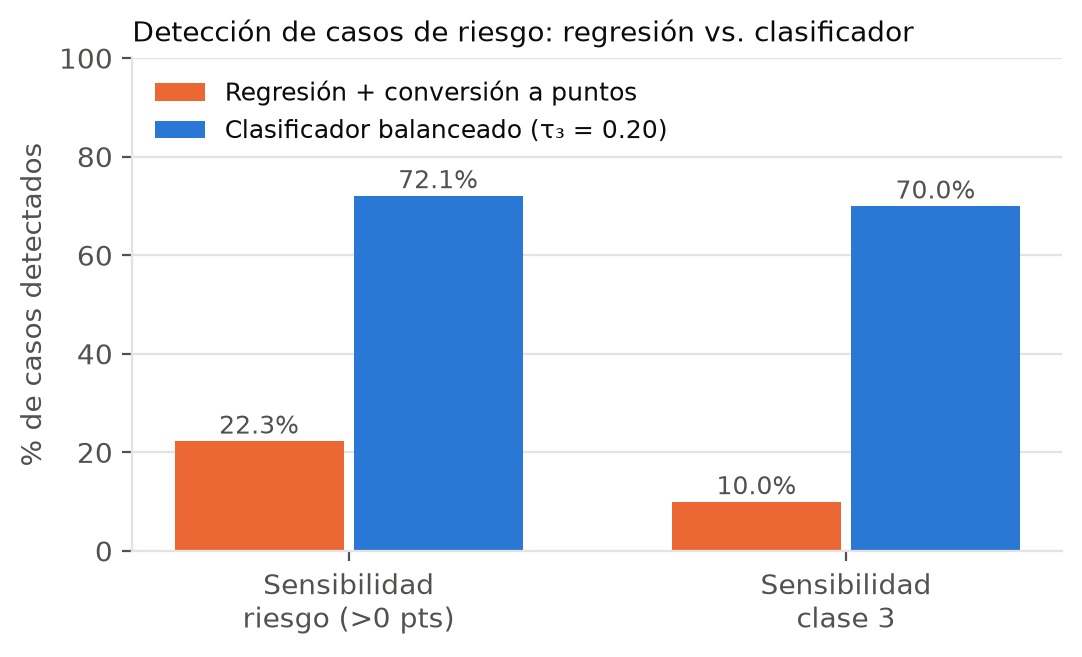
\includegraphics[width=0.7\linewidth]{res_regresion_vs_clasificador.png}
    \caption{Sensibilidad para detectar casos de riesgo con el enfoque de regresión y con el clasificador balanceado.}
    \label{fig:reg_vs_clf}
\end{figure}

La Figura \ref{fig:confusion} presenta la matriz de confusión del clasificador sobre el conjunto de prueba con la regla argmax, normalizada por fila. Con esta regla el modelo obtiene una exactitud de 74.5\% en las cuatro clases y de 92.7\% con tolerancia de $\pm 1$ punto. Los errores se concentran entre clases vecinas, que tienen poco efecto sobre el puntaje NEWS-2 total, y la clase 3 alcanza una sensibilidad de 54.6\%. El 19.7\% de los casos de 3 puntos se clasifican como normales, lo cual motivó el ajuste del umbral de esta clase.

\begin{figure}[H]
    \centering
    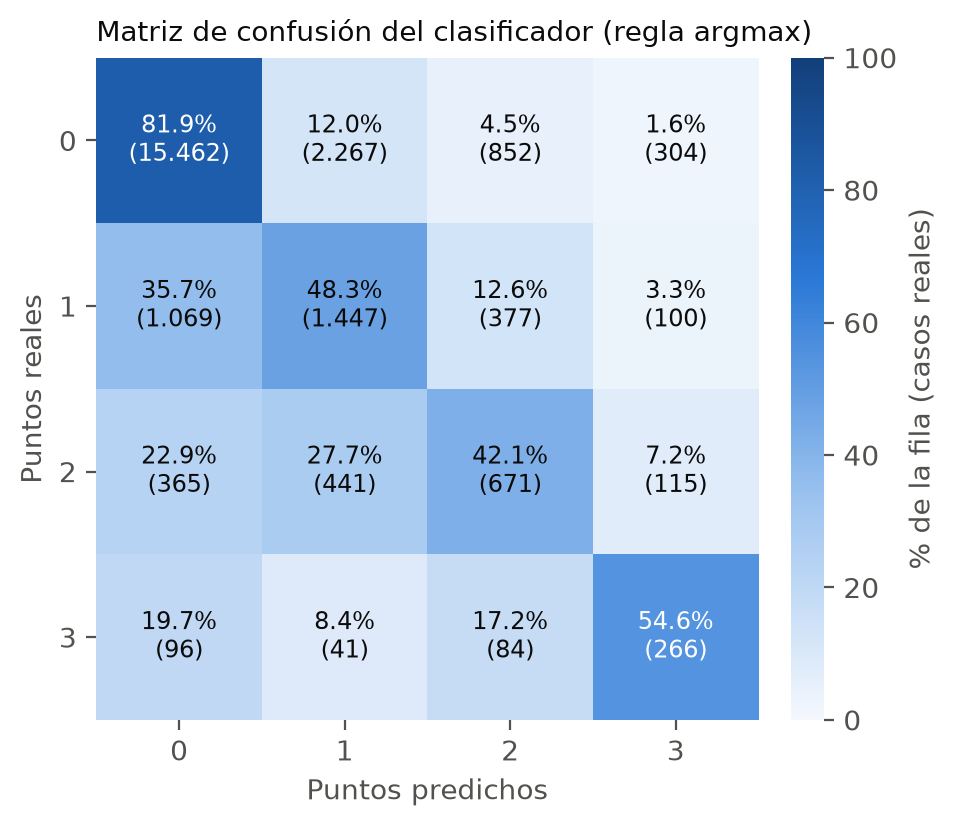
\includegraphics[width=0.6\linewidth]{res_matriz_confusion.png}
    \caption{Matriz de confusión del clasificador en el conjunto de prueba (regla argmax), normalizada por fila.}
    \label{fig:confusion}
\end{figure}

La Figura \ref{fig:umbral} muestra el efecto del umbral $\tau_3$ sobre la sensibilidad de la clase 3 y sobre la proporción de casos normales clasificados como 3 puntos. Al bajar el umbral aumenta la detección de casos severos, pero por debajo de 0.20 las falsas alarmas crecen rápidamente (11.4\% con 0.15 y 22.6\% con 0.10). Con el umbral elegido de 0.20 la sensibilidad de la clase 3 sube de 54.6\% a 70.0\% mientras que la proporción de falsos casos de 3 puntos se mantiene en 6.1\%. La Tabla \ref{tab:metricas_finales} resume las métricas del modelo final.

\begin{figure}[H]
    \centering
    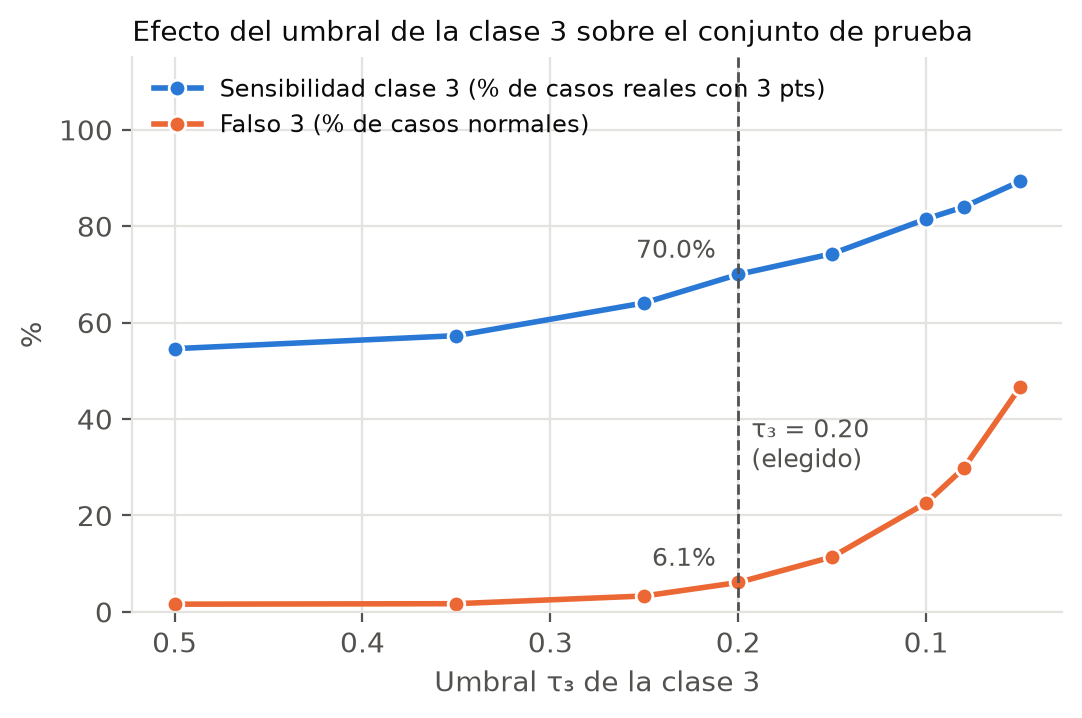
\includegraphics[width=0.7\linewidth]{res_umbral.png}
    \caption{Sensibilidad de la clase 3 y tasa de falsos casos de 3 puntos en función del umbral $\tau_3$.}
    \label{fig:umbral}
\end{figure}

\begin{table}[H]
\centering
\begin{tabular}{lcc}
\toprule
\textbf{Métrica} & \textbf{Argmax} & \textbf{Regla final ($\tau_3 = 0.20$)} \\
\midrule
Sensibilidad clase 3 & 54.6\% & 70.0\% \\
Falsos casos de 3 puntos (\% de normales) & 1.6\% & 6.1\% \\
Sensibilidad de riesgo ($>0$ puntos) & 69.8\% & 72.1\% \\
\bottomrule
\end{tabular}
\caption{Métricas del clasificador en el conjunto de prueba.}
\label{tab:metricas_finales}
\end{table}

\subsection{Discusión}

El aspecto más relevante del trabajo es la reformulación del problema de presión arterial. Los experimentos demostraron que, con un solo sensor PPG y sin calibración, no es posible estimar la presión en mmHg con precisión clínica, y que esta limitación proviene de la información disponible en la señal y no del modelo. En lugar de reportar un valor en mmHg poco confiable, el sistema clasifica directamente el nivel de riesgo que requiere la escala NEWS-2, lo cual triplicó la detección de casos de riesgo y permite incorporar la presión al puntaje sin \textit{hardware} adicional. La regla de decisión se ajustó al uso real de la salida, priorizando los casos de 3 puntos, que son los únicos que por sí solos activan la respuesta urgente de la escala.

Desde el punto de vista de la arquitectura, el procesamiento en el borde permitió que toda la analítica, incluido el modelo, se ejecute en la Raspberry Pi 3 y que la nube solo almacene y distribuya los resultados. La separación en dos hilos fue necesaria para no perder muestras del sensor, y el uso de SenML, MQTT sobre TLS y la reconstrucción de los campos en la aplicación permitieron trabajar dentro de los límites de la versión gratuita de ThingSpeak.

Las principales limitaciones identificadas son: las métricas del modelo se obtuvieron con una separación por registro y no por paciente, ya que el \textit{dataset} no incluye el identificador de paciente; el modelo fue entrenado con señales de monitores clínicos y se aplica sobre un sensor de bajo costo, por lo que su desempeño en operación puede diferir del obtenido en prueba; y las lecturas de temperatura, SpO\textsubscript{2} y frecuencia respiratoria requieren calibración, ya que en las pruebas generaron alertas sin un deterioro real. Por estas razones, VIGIA se presenta como una herramienta de alerta temprana de tendencia que apoya la vigilancia del personal médico, y no como un instrumento de medición clínica.

% ------------------------------------------------------------
\section{Conclusiones}\label{sec:conclusiones}

\begin{itemize}
    \item Se implementó una solución IoT de extremo a extremo para el monitoreo de signos vitales y el cálculo automático de la escala NEWS-2, compuesta por un nodo basado en Raspberry Pi 3 con los sensores MAX30100 y MLX90614, transmisión por MQTT sobre TLS hacia ThingSpeak y una aplicación Android que presenta el estado del paciente y genera la alerta crítica. Las pruebas confirmaron el funcionamiento de toda la cadena, desde la lectura de los sensores hasta la alerta en el teléfono.

    \item A partir de una única señal PPG fue posible obtener cuatro de los parámetros de la escala: frecuencia cardíaca, saturación de oxígeno, frecuencia respiratoria y nivel de riesgo de la presión arterial sistólica. Esto reduce el \textit{hardware} necesario a dos sensores de bajo costo, en lugar de un monitor de cabecera.

    \item Los experimentos demostraron que estimar la presión sistólica en mmHg con PPG de un solo sensor y sin calibración no cumple el estándar AAMI (desviación estándar del error de 16.68~mmHg frente al límite de 8~mmHg), y que esta limitación se debe a un sesgo propio de cada paciente y no a la capacidad del modelo ni a la cantidad de datos. Una calibración por paciente reduciría el error hasta casi cumplir el estándar, pero requiere un tensiómetro.

    \item Reformular el problema como la clasificación directa de los puntos NEWS-2 de presión, con pesos balanceados por clase y un umbral de decisión de 0.20 para la clase de 3 puntos, elevó la sensibilidad para detectar casos de riesgo de 22.3\% a 72.1\% y la de los casos de 3 puntos de 10.0\% a 70.0\%, con una tasa de falsos casos de 3 puntos de 6.1\%. Ajustar la salida del modelo a la decisión clínica que debe apoyar resultó más útil que buscar un valor numérico poco confiable.

    \item El procesamiento en el borde permitió ejecutar toda la analítica, incluido el modelo, en la Raspberry Pi 3, dejando a la nube solo el almacenamiento y la distribución de los datos. La separación del código en dos hilos fue indispensable para no perder muestras del MAX30100, cuya FIFO solo almacena 160~ms de señal.

    \item La versión gratuita de ThingSpeak limita la escritura a un mensaje cada 15 segundos, lo cual hace que cada variable se actualice cada 160 segundos aproximadamente. Esta latencia es adecuada para el seguimiento de tendencias que propone NEWS-2, pero no para un monitoreo continuo en tiempo real.

    \item La confiabilidad de la alerta depende de la calidad de cada medición. Las lecturas de temperatura, SpO\textsubscript{2} y frecuencia respiratoria generaron alertas sin un deterioro real, por lo que su calibración contra instrumentos de referencia es el paso necesario antes de cualquier uso clínico. Como trabajo futuro se proponen además validar el clasificador con datos adquiridos con el propio MAX30100, separar los datos por paciente en la evaluación, notificar las alertas aunque la aplicación esté cerrada y migrar a una plataforma sin el límite de escritura de ThingSpeak.
\end{itemize}


\newpage

% ------------------------------------------------------------
% REFERENCIAS EN FORMATO IEEE
% ------------------------------------------------------------



\begin{thebibliography}{99}

\bibitem{ref5}
GT-LATINFURG, ``Recomendaciones del GT-LATINFURG para la identificación y atención inicial del paciente con infección grave y sepsis en los servicios de urgencias,'' \textit{Revista Emergencias}. [Online]. Available: \url{https://revistaemergencias.org/articulo/recomendaciones-para-la-identificacion-y-atencion-inicial-del-paciente-con-infeccion-grave-y-sepsis-en-los-servicios-de-urgencias-del-gt-latinfurg/}

\bibitem{ref6}
L. Mellhammar et al., ``NEWS2 is superior to qSOFA in detecting sepsis with organ dysfunction in the emergency department,'' \textit{J. Clin. Med.}, vol. 8, no. 8, p. 1128, 2019, doi: 10.3390/jcm8081128.

\bibitem{ref7}
O. A. Usman, A. A. Usman, and M. A. Ward, ``Comparison of SIRS, qSOFA, and NEWS for the early identification of sepsis in the Emergency Department,'' \textit{Am. J. Emerg. Med.}, vol. 37, no. 8, pp. 1490--1497, 2019.

\bibitem{ref8}
M. M. Churpek et al., ``Quick Sepsis-related Organ Failure Assessment, Systemic Inflammatory Response Syndrome, and Early Warning Scores for detecting clinical deterioration in infected patients outside the intensive care unit,'' \textit{Am. J. Respir. Crit. Care Med.}, vol. 195, no. 7, pp. 906--911, 2017.

\bibitem{ref9}
A. F. Oduncu, G. S. Kıyan, and S. Yalçınlı, ``Comparison of qSOFA, SIRS, and NEWS scoring systems for diagnosis, mortality, and morbidity of sepsis in emergency department,'' \textit{Am. J. Emerg. Med.}, vol. 48, pp. 54--59, 2021, doi: 10.1016/j.ajem.2021.04.006.

\bibitem{ref10}
L. Evans et al., ``Surviving Sepsis Campaign: International Guidelines for Management of Sepsis and Septic Shock 2021,'' \textit{Intensive Care Med.}, vol. 47, pp. 1181--1247, 2021, doi: 10.1007/s00134-021-06506-y.

\bibitem{ref16}
E. L'Her, Q.-T. N'Guyen, V. Pateau, L. Bodenes, and F. Lellouche, ``Photoplethysmographic determination of the respiratory rate in acutely ill patients: validation of a new algorithm and implementation into a biomedical device,'' \textit{Ann. Intensive Care}, vol. 9, no. 1, p. 11, 2019, doi: 10.1186/s13613-019-0485-z.

\bibitem{ref12}
Y.-C. Hsu, Y.-H. Li, C.-C. Chang, and L. N. Harfiya, ``Generalized deep neural network model for cuffless blood pressure estimation with photoplethysmogram signal only,'' \textit{Sensors}, vol. 20, no. 19, p. 5668, 2020, doi: 10.3390/s20195668.

\bibitem{ref13}
N. Ibtehaz and M. S. Rahman, ``PPG2ABP: Translating photoplethysmogram (PPG) signals to arterial blood pressure (ABP) waveforms,'' \textit{Bioengineering}, vol. 9, no. 11, p. 692, 2022, doi: 10.3390/bioengineering9110692.

\bibitem{ref14}
C. Wang, F. Yang, X. Yuan, Y. Zhang, K. Chang, and Z. Li, ``An end-to-end neural network model for blood pressure estimation using PPG signal,'' in \textit{Artificial Intelligence in China}, Singapore: Springer, 2020, pp. 262--272, doi: 10.1007/978-981-15-3514-7\_21.

\bibitem{ref15}
X. Chen, S. Yu, Y. Zhang, F. Chu, and B. Sun, ``Machine learning method for continuous noninvasive blood pressure detection based on random forest,'' \textit{IEEE Access}, vol. 9, 2021, doi: 10.1109/ACCESS.2021.3062033.

\bibitem{ref17}
K. Dheman, M. Giordano, C. Thomas, P. Schilk, and M. Magno, ``i-CardiAx: Wearable IoT-driven system for early sepsis detection through long-term vital sign monitoring,'' \textit{arXiv:2407.21433}, 2024. [Online]. Available: \url{https://arxiv.org/abs/2407.21433}

\bibitem{ref18}
A. J. Singh, J. Gnanasoundharam, M. Birunda, G. Sudha, S. P. Maniraj, and C. Srinivasan, ``Wearable sepsis early warning using cloud computing and logistic regression predictive analytics,'' in \textit{Proc. 2024 11th Int. Conf. on Reliability, Infocom Technologies and Optimization (Trends and Future Directions) (ICRITO)}, Noida, India, 2024, pp. 1--6, doi: 10.1109/ICRITO61523.2024.10522250.

\bibitem{ref19}
F. Mahmud, M. Quamruzzaman, A. I. Sanka, R. C. C. Cheung, and M. H. Chowdhury, ``Interpretable machine learning-based real-time sepsis diagnosis,'' \textit{Scientific Reports}, 2026. [Online]. Available: \url{https://www.nature.com/articles/s41598-026-36945-w}

\bibitem{ref20}
Y.-S. Chen, W.-H. Wang, C.-T. Hu, and I. You, ``Cross-modal contrastive learning for predicting sepsis onset in Medical Internet of Things (MIoT),'' \textit{Internet of Things}, vol. 29, p. 101456, 2025.

\bibitem{ref21}
S. Ghiasi, T. Zhu, P. Lu, J. Hagenah, P. N. Q. Khanh, N. Van Hao, L. Thwaites, D. A. Clifton, and Vital Consortium, ``Sepsis Mortality Prediction Using Wearable Monitoring in Low--Middle Income Countries,'' \textit{Sensors}, vol. 22, no. 10, p. 3866, 2022. [Online]. Available: \url{https://www.mdpi.com/1424-8220/22/10/3866}

\bibitem{ref1}
World Health Organization, ``Sepsis,'' May 3, 2024. [Online]. Available: \url{https://www.who.int/news-room/fact-sheets/detail/sepsis}

\bibitem{ref2}
J. F. Martín-Ramírez, A. Domínguez-Borgua, and A. D. Vázquez-Flores, ``Sepsis,'' \textit{Med. Int. Méx.}, vol. 30, no. 2, pp. 159--175, 2014.

\bibitem{ref3}
``Epidemiología de la sepsis en unidades de cuidado intensivo en Colombia,'' \textit{Biomédica}. [Online]. Available: \url{https://revistabiomedica.org/index.php/biomedica/article/view/1439/2342}

\bibitem{ref4}
Y. Pertuz-Meza, C. Pérez-Quintero, and Y. Pabón-Varela, ``Aspectos epidemiológicos de la sepsis, en unidades de cuidados intensivos Santa Marta, Colombia,'' \textit{Duazary}, vol. 13, no. 2, pp. 126--132, 2016, doi: 10.21676/2389783X.1718.

\bibitem{ref22}
M. Kachuee, M. M. Kiani, H. Mohammadzade, and M. Shabany, ``Cuff-Less Blood Pressure Estimation,'' UCI Machine Learning Repository, 2015. [Online]. Available: \url{https://archive.ics.uci.edu/dataset/340/cuff+less+blood+pressure+estimation}

\bibitem{ref23}
ANSI/AAMI/ISO 81060-2:2018, ``Non-invasive sphygmomanometers -- Part 2: Clinical investigation of intermittent automated measurement type,'' Association for the Advancement of Medical Instrumentation, Arlington, VA, 2018.

\bibitem{ref26}
Royal College of Physicians, ``National Early Warning Score (NEWS) 2: Standardising the assessment of acute-illness severity in the NHS,'' London: RCP, 2017.

\bibitem{ref24}
S. Samimi and H. R. Dajani, ``A PPG-Based Calibration-Free Cuffless Blood Pressure Estimation Method Using Cardiovascular Dynamics,'' \textit{Sensors}, vol. 23, no. 8, p. 4145, 2023, doi: 10.3390/s23084145.

\bibitem{ref25}
J. Joung et al., ``Continuous cuffless blood pressure monitoring using photoplethysmography-based PPG2BP-net for high intrasubject blood pressure variations,'' \textit{Scientific Reports}, vol. 13, 2023, doi: 10.1038/s41598-023-35492-y.

\end{thebibliography}

\end{document}
